%%
%% This is file `sample-authordraft.tex',
%% generated with the docstrip utility.
%%
%% The original source files were:
%%
%% samples.dtx  (with options: `authordraft')
%% 
%% IMPORTANT NOTICE:
%% 
%% For the copyright see the source file.
%% 
%% Any modified versions of this file must be renamed
%% with new filenames distinct from sample-authordraft.tex.
%% 
%% For distribution of the original source see the terms
%% for copying and modification in the file samples.dtx.
%% 
%% This generated file may be distributed as long as the
%% original source files, as listed above, are part of the
%% same distribution. (The sources need not necessarily be
%% in the same archive or directory.)
%%
%% The first command in your LaTeX source must be the \documentclass command.
% \documentclass[sigconf,authordraft]{acmart}


%%%% As of March 2017, [siggraph] is no longer used. Please use sigconf (above) for SIGGRAPH conferences.

%%%% As of May 2020, [sigchi] and [sigchi-a] are no longer used. Please use sigconf (above) for SIGCHI conferences.

%%%% Proceedings format for SIGPLAN conferences 
% \documentclass[sigplan, anonymous, authordraft]{acmart}

%%%% Proceedings format for conferences using one-column small layout
\documentclass[sigconf]{acmart} %acmsmall

% NOTE that a single column version is required for submission and peer review. This can be done by changing the \doucmentclass[...]{acmart} in this template to 
% \documentclass[manuscript,screen]{acmart}

%%
%% \BibTeX command to typeset BibTeX logo in the docs
\AtBeginDocument{%
  \providecommand\BibTeX{{%
    \normalfont B\kern-0.5em{\scshape i\kern-0.25em b}\kern-0.8em\TeX}}}

%% Rights management information.  This information is sent to you
%% when you complete the rights form.  These commands have SAMPLE
%% values in them; it is your responsibility as an author to replace
%% the commands and values with those provided to you when you
%% complete the rights form.
\usepackage{booktabs} % For formal tables
\usepackage{listings}
\usepackage{amsmath}
\usepackage{amssymb}
\usepackage{graphicx}
\usepackage{setspace}
\usepackage{fullpage}
\usepackage{xcolor}
\usepackage{caption}
\usepackage{program}
\usepackage{epstopdf}
\usepackage{algorithm}
% \usepackage{indentfirst}
\usepackage{algorithmicx}
\usepackage{algpseudocode}
\usepackage{subfigure}
\usepackage{courier}
\usepackage{enumitem}
\usepackage{comment}
\usepackage[font=normal,skip=0pt]{caption}
\usepackage{xspace}


\setcopyright{acmcopyright}
\copyrightyear{2018}
\acmYear{2018}
\acmDOI{10.1145/1122445.1122456}

%% These commands are for a PROCEEDINGS abstract or paper.
\acmConference[Woodstock '18]{Woodstock '18: ACM Symposium on Neural
  Gaze Detection}{June 03--05, 2018}{Woodstock, NY}
\acmBooktitle{Woodstock '18: ACM Symposium on Neural Gaze Detection,
  June 03--05, 2018, Woodstock, NY}
\acmPrice{15.00}
\acmISBN{978-1-4503-XXXX-X/18/06}


\DeclareRobustCommand{\system}{\mbox{\scshape System-X}\xspace}
\DeclareRobustCommand{\company}{\mbox{\scshape Company-X}\xspace}
\DeclareRobustCommand{\vta}{\mbox{\scshape VTA}\xspace}
\DeclareRobustCommand{\vita}{\mbox{\scshape VITA}\xspace}
\DeclareRobustCommand{\vital}{\mbox{\scshape VITAL}\xspace}
\DeclareRobustCommand{\vitaframe}{\mbox{\scshape VITAframe}\xspace}
\DeclareRobustCommand{\subhead}[1]{\noindent\textbf{#1}} 

\newenvironment{paraenum}{\begin{inparaenum}[\itshape (a)\upshape]}{\end{inparaenum}}
\newcommand{\stitle}[1]{\vspace{0.2em}\noindent\textbf{#1}}
\newcommand{\etitle}[1]{\vspace{0.2em}\noindent{\emph{#1}}}
\newcommand{\emtitle}[1]{\vspace{0.15em}\noindent\underline{\em #1}}
\newcommand{\hide}[1]{}
\newcommand{\saj}[1]{\textcolor{teal}{#1}}
\newcommand{\peter}[1]{\textcolor{blue}{#1}}
\newcommand{\candidate}[1]{} %\textcolor{orange}{#1}
\newcommand{\sajreview}[1]{{#1}}
\definecolor{corange}{HTML}{C31D00}
\newcommand{\creview}[1]{\textcolor{corange}{#1}}
\newcommand{\todo}[1]{\textcolor{red}{#1}}
\newcommand{\eg}{{\itshape e.g.}, }
\newcommand{\ie}{{\itshape i.e.}, }
\newcommand{\ta}[1]{\begin{framed}\vspace{-3pt}\noindent\textit{#1}\vspace{-3pt}\end{framed}}
\newcommand{\boxy}[1]{\vspace{-3pt}\begin{framed}\vspace{-5pt}\noindent#1\vspace{-7pt}\end{framed}\vspace{-5pt}}
\newcommand{\squishlist}{
  \begin{list}{$\bullet$}
           { \setlength{\itemsep}{0pt}
             \setlength{\parsep}{2pt}
             \setlength{\topsep}{2pt}
             \setlength{\partopsep}{0pt}
           }
}
\newcommand{\squishend}{\end{list}}


\newcommand{\squishenum}{
       \begin{enumerate}
               { \setlength{\itemsep}{-50pt}
                       \setlength{\parsep}{0pt}
                       \setlength{\topsep}{0pt}
                       \setlength{\partopsep}{0pt}
               }
       }
\newcommand{\squishenumend}{\end{enumerate}}

\newtheorem{definition}{Definition}
\newtheorem{problem}{Problem}

\newcommand{\code}[1]{\texttt{\small #1}}





%%
%% Submission ID.
%% Use this when submitting an article to a sponsored event. You'll
%% receive a unique submission ID from the organizers
%% of the event, and this ID should be used as the parameter to this command.
%%\acmSubmissionID{123-A56-BU3}

%%
%% The majority of ACM publications use numbered citations and
%% references.  The command \citestyle{authoryear} switches to the
%% "author year" style.
%%
%% If you are preparing content for an event
%% sponsored by ACM SIGGRAPH, you must use the "author year" style of
%% citations and references.
%% Uncommenting
%% the next command will enable that style.
%%\citestyle{acmauthoryear}

%%
%% end of the preamble, start of the body of the document source.
\begin{document}

%%
%% The "title" command has an optional parameter,
%% allowing the author to define a "short title" to be used in page headers.
\title{Towards integrated, interactive, and extensible text data analytics with \system}

%%
%% The "author" command and its associated commands are used to define
%% the authors and their affiliations.
%% Of note is the shared affiliation of the first two authors, and the
%% "authornote" and "authornotemark" commands
%% used to denote shared contribution to the research.
% \author{Ben Trovato}
% \authornote{Both authors contributed equally to this research.}
% \email{trovato@corporation.com}
% \orcid{1234-5678-9012}
% \author{G.K.M. Tobin}
% \authornotemark[1]
% \email{webmaster@marysville-ohio.com}
% \affiliation{%
%   \institution{Institute for Clarity in Documentation}
%   \streetaddress{P.O. Box 1212}
%   \city{Dublin}
%   \state{Ohio}
%   \postcode{43017-6221}
% }

% \author{Lars Th{\o}rv{\"a}ld}
% \affiliation{%
%   \institution{The Th{\o}rv{\"a}ld Group}
%   \streetaddress{1 Th{\o}rv{\"a}ld Circle}
%   \city{Hekla}
%   \country{Iceland}}
% \email{larst@affiliation.org}

% \author{Valerie B\'eranger}
% \affiliation{%
%   \institution{Inria Paris-Rocquencourt}
%   \city{Rocquencourt}
%   \country{France}
% }

% \author{Aparna Patel}
% \affiliation{%
%  \institution{Rajiv Gandhi University}
%  \streetaddress{Rono-Hills}
%  \city{Doimukh}
%  \state{Arunachal Pradesh}
%  \country{India}}

% \author{Huifen Chan}
% \affiliation{%
%   \institution{Tsinghua University}
%   \streetaddress{30 Shuangqing Rd}
%   \city{Haidian Qu}
%   \state{Beijing Shi}
%   \country{China}}

% \author{Charles Palmer}
% \affiliation{%
%   \institution{Palmer Research Laboratories}
%   \streetaddress{8600 Datapoint Drive}
%   \city{San Antonio}
%   \state{Texas}
%   \postcode{78229}}
% \email{cpalmer@prl.com}

% \author{John Smith}
% \affiliation{\institution{The Th{\o}rv{\"a}ld Group}}
% \email{jsmith@affiliation.org}

% \author{Julius P. Kumquat}
% \affiliation{\institution{The Kumquat Consortium}}
% \email{jpkumquat@consortium.net}

%%
%% By default, the full list of authors will be used in the page
%% headers. Often, this list is too long, and will overlap
%% other information printed in the page headers. This command allows
%% the author to define a more concise list
%% of authors' names for this purpose.
%\renewcommand{\shortauthors}{Trovato and Tobin, et al.}
\settopmatter{printfolios=true} 
%%
%% The abstract is a short summary of the work to be presented in the
%% article.
\begin{abstract}
From tweets to product reviews, text is ubiquitous on the web and often contains highly valuable information for both enterprises and consumers. However, online text is generally noisy and incomplete, requiring adequate extensible tools for iterative, integrated text analysis and mining.  While there are systems effective for different stages of text analysis, users lack extensible 
platforms to support interactive text analysis 
workflows end-to-end. Here we introduce \system combining the strengths of spreadsheets, computational notebooks, and interactive visualizations to facilitate integrated text analytics. \system implements a visual text algebra to facilitate extensible and expressive analysis, supporting diverse tasks ranging from data cleaning to visualization. It also enables declarative specification of interactive coordination across views of data, code, and visualizations. We evaluate \system through two case studies using two popular Kaggle text analytics workflows and elicit user feedback. Based on our findings, we discuss the implications and opportunities for integrated text analysis.

% From tweets to online product reviews, digital text on the web is ubiquitous. Text analysis often involves multiple tasks---data wrangling, model building, hypothesis testing, insight extraction---which analysts perform in an iterative, non-linear fashion. While there are many systems like spreadsheets, computational notebooks, and visualization tools to support many of these tasks, there is a lack of an integrated analytics platform to support an entire text analysis workflow. We propose \system that provides a multiple-coordinated interface featuring data, script, and chart views. \system allows analysts to manipulate, model, and analyze text datasets via scripts and GUI-based operators while enabling coordinated data exploration. The analysis and coordination operators are developed based on an existing visual text algebra. We test \system on two case studies with researchers at \company and obtain feedback on the its pros and cons. Based on our findings, we discuss the implications and opportunities for integrated text analysis.


% \begin{comment}
% With the increase in scale and availability of digital text generated on the web, enterprises such as online retailers and aggregators often use text analytics to mine and analyze the data to improve their services and products alike. 
% Text data analysis is an iterative, non-linear process with diverse workflows spanning multiple stages, from data cleaning to visualization. Existing text analytics systems usually accommodate a subset of these stages and often fail to address challenges related to data heterogeneity, provenance, workflow reusability and reproducibility, and compatibility with established practices.  Based on a set of design considerations we derive from these challenges, we propose \system, a system that treats the text analysis process as a single continuum by combining advantages of computational notebooks, spreadsheets, and visualization tools. \system features an interactive user interface for running text analysis workflows, a new data model for managing multiple atomic and composite data types, and an expressive algebra that captures diverse sets of operations representing various stages of text analysis and enables coordination among different components of the system,  including data, code, and visualizations. We report our current progress in \system development while demonstrating its usefulness with usage examples. Finally, we outline a number of enhancements to \system and identify several research directions for developing an interactive visual text analysis system.
% \end{comment}




\end{abstract}

%%
%% The code below is generated by the tool at http://dl.acm.org/ccs.cfm.
%% Please copy and paste the code instead of the example below.
%%
\begin{CCSXML}
<ccs2012>
<concept>
<concept_id>10003120.10003121</concept_id>
<concept_desc>Human-centered computing~Interactive systems and tools</concept_desc>
<concept_significance>500</concept_significance>
</concept>
</ccs2012>
\end{CCSXML}

\ccsdesc[500]{Human-centered computing~Interactive systems and tools}

%%
%% Keywords. The author(s) should pick words that accurately describe
%% the work being presented. Separate the keywords with commas.
\keywords{Interactive text analysis, text data management, text algebra.}

%% A "teaser" image appears between the author and affiliation
%% information and the body of the document, and typically spans the
%% page.

%%
%% This command processes the author and affiliation and title
%% information and builds the first part of the formatted document.
\maketitle

 
\begin{figure}[tbp] 
  \centering
  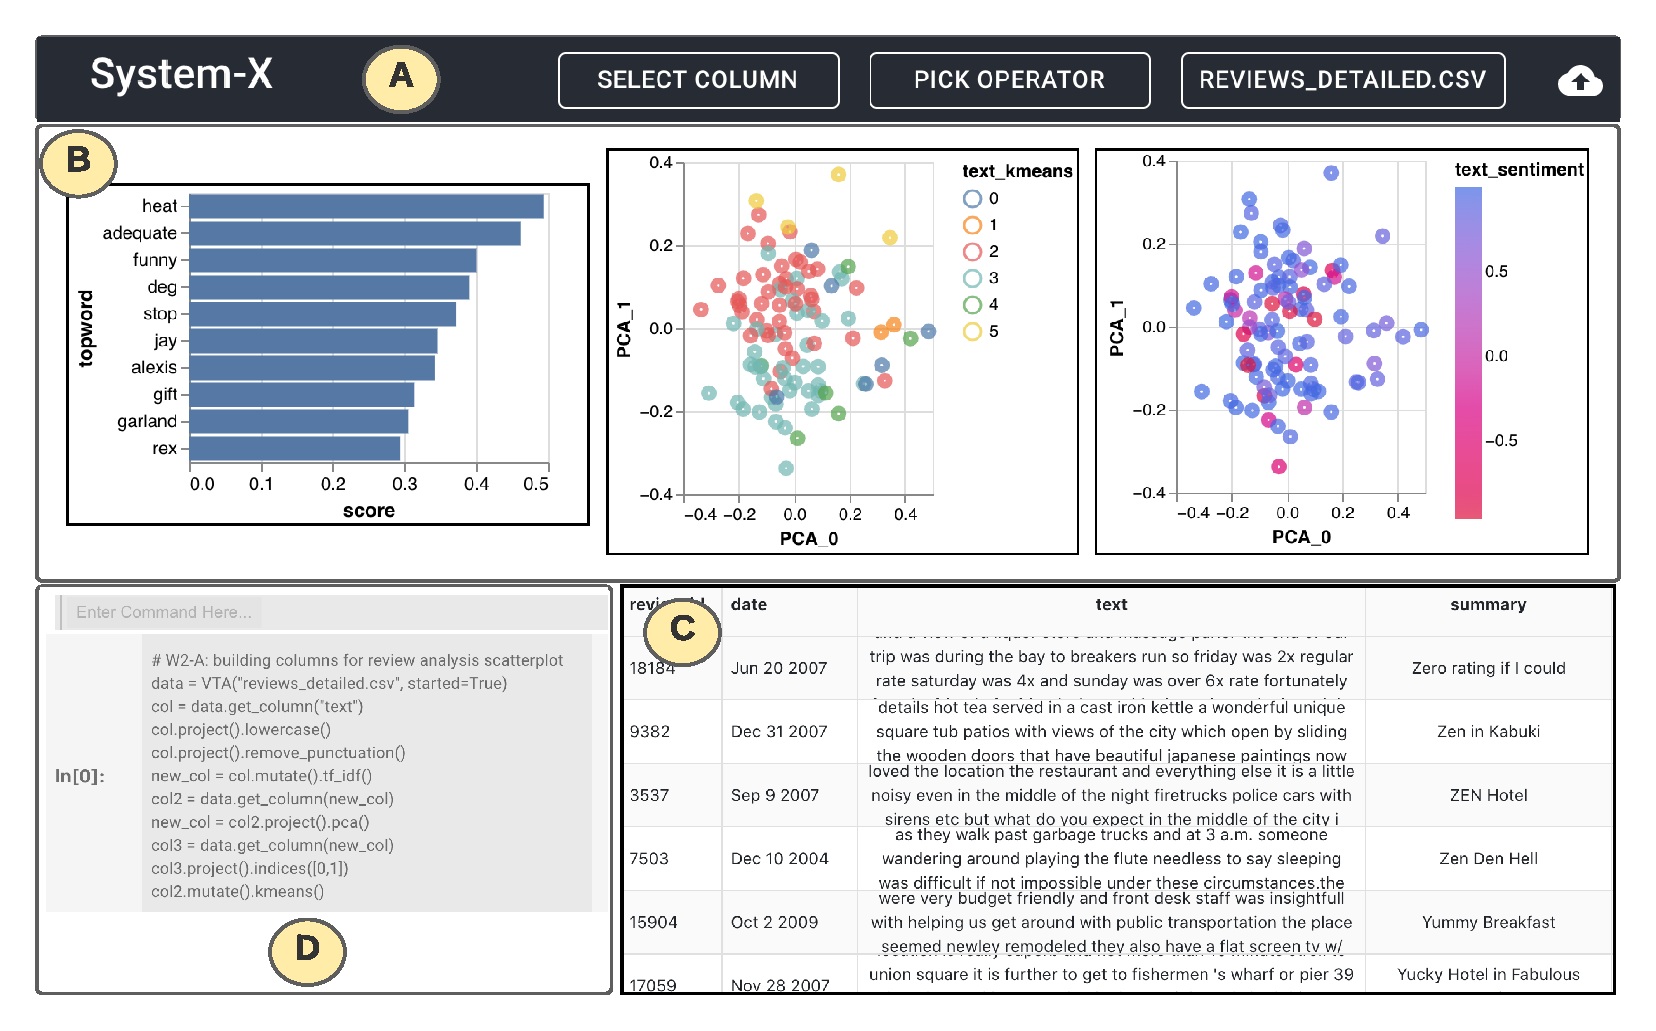
\includegraphics[width=\linewidth]{figures/leam_fe.pdf}
  \caption{\small \system user interface. (A) Operator View enables users to perform visual text analytics (\vita) operations using drop-down menus, (B) Visualization View 
  holds a carousel of interactive visualizations created by users, (C) Table View displays the data and its subsequent transformations, and (D) Notebook View allows users to compose and run \vita operations using a declarative language. Inset (E) shows the \vta JSON specification for the bar chart operator in Operator View. Inset (F) shows a declarative \vta command for interacting with the bar chart from Notebook View. \label{fig:fe}} 
\end{figure}

\section{Introduction}\label{sec:intro}
% motivate the problem space and its relevance and impact 
The internet has become the platform for many of our everyday activities, from shopping to dating. The global market size of e-commerce has exponentially increased in the last decade. 
The upward trend is expected to be continued.  A recent study projects the worldwide e-commerce sales to be around six trillion dollars by 2023~\cite{ecommerce}, nearly a 50\% increase over the current market. This growth has contributed to the proliferation of digital text, particularly user-generated text (reviews, Q\&As, discussions), which often contain useful information for improving the services and products on the web. Enterprises increasingly adopt text mining technologies to extract, analyze, and summarize information from such unstructured text data.

% online text is noisy in many senses, which warrants systems taking integrative 
% approach to their analysis 
However, online text collections are notoriously noisy, incomplete, ambiguous, subjective and often sparse in informational content. Consider reviews; a review about a hotel, for example, typically refers to only a few qualities about the hotel, such as location and service, out of many possible.  Discovering, cleaning, analyzing, searching, modeling, extracting information from, and identifying and exploring topics in such text collections can be daunting and time consuming without integrated systems that take the whole text analytics pipeline 
into account. 

The characteristics of online text make interactive workflows and visualizations not only appealing but also essential for accessible, rapid iterative analysis~\cite{ittoo2016text}.
Therefore we here focus on visual interactive text analysis (\vita hereafter) and related systems. There are a few commercial (e.g.,~\cite{sastextminer,rapidminer,tableau,powerbi}) 
and open-source tools (e.g.,\cite{perez2007ipython,nltk,gensim,spacy}) that can  support different stages of \vita at varying degrees~\cite{liu2018bridging, mlbazaar}. For example, spreadsheets allow directly processing and manipulating  data, computational notebooks enable flexible exploratory analysis and modeling, and visualization systems, typically based on chart templates, facilitate quick interactive visual analysis.  An ideal system would unify these affordances~\cite{kandel2011research,drosos2020wrex,wu2020b2}.  There are also many customized visual text analytics tools~\cite{liu2018bridging}, often in the form of research prototypes, that focus on specific use-cases like review exploration~\cite{zhang2020teddy}, sentiment analysis~\cite{kucher2018state}, and text summarization~\cite{carenini2006interactive}.
Unfortunately, none of these solutions accommodate the inherently cyclic, 
trial-and-error-based nature of \vita pipelines end to end in an integrated manner. 


\todo{Expand and revise to answer the question: Why is it difficult to develop an end-to-end \vita system?} 
\vita is an iterative and non-linear process---it is a multistage process that involves tasks like data preprocessing and transformation, model building, hypothesis testing, and insight exploration, all of which require multiple iterations to obtain satisfactory outcomes. While having end-to-end  \vita systems is much desired, designing and building them is difficult. The primary 
   challenge is the number and diversity of the tasks that need to be supported. In part, 
   programmatic tools such as computational notebooks can provide extensibility and 
   expressivity to incrementally build such support but they often lack in interactivity, 
   accessibility, and scalability, impeding non-linear iterative analysis. 

%  :  (a) extensibility and expressivity of \vita workflows, (b) their continuity and reproducibility, (c) data heterogeneity and provenance, and (d) coordination  of user interactions.  The challenges identified here are informed by our experience in developing data systems, working with practitioners as part of an industry research lab, part of a larger company with more than three hundred e-commerce subsidiaries and prior research, particularly those  reporting from interview studies on data analysis workflows~\cite{zhang2020teddy,lee2020demystifying},

\todo{Revise and complete. BTW, `one-stop-shop' might  offend some reviewers. } 
In response, we propose \system, a one-stop-shop for visual interactive text analysis. \system combines the advantages of spreadsheets, computational notebooks, and visualization tools by integrating a Notebook View with interactive views of raw and transformed data (Figure~\ref{fig:fe}). A key component in the design of \system is a visual text algebra (\vta) that enables users to specify complex \vita operations over heterogeneous data and their visual representations; either using a declarative language in the Notebook View (Figure~\ref{fig:fe}F) or by creating operators in the front-end that translates to \vta specifications (Figure~\ref{fig:fe}E) in JSON (JavaScript Object Notation). Through usage examples, we demonstrate the expressivity of \vta and how it enables \system to support diverse tasks ranging from data cleaning to visualization. Moreover, to facilitate efficient execution of \vta on heterogeneous data, we introduce a new data model extending dataframes called \vitaframe.
To evaluate \system, we conduct two case studies using two popular Kaggle text 
analytics workflows for tweet analysis and spam detection, respectively, and elicit 
user feedback. Our findings suggest \system is $\ldots$. We have made the current 
version of \system open-source at~\url{https://github.com/chi-author/system-x}.


\section{Related Work}\label{sec:related}

We now summarize existing work on interactive text analysis and visualization, text analysis libraries and frameworks, workflow and task specification for text analysis, and programming environments for data analysis.

\stitle{Domain-specific text analysis tools.}
There are many commercial tools and research prototypes 
that provide direct manipulation interfaces to help users
create specific types of text analysis application:
sentiment analysis~\cite{zhao2014pearl,wang2015senticompass,brooks2014collaborative} and opinion mining~\cite{miao2009amazing,wu2010opinionseer,mahmud2016predicting}, 
question answering~\cite{shen2015word,gordon2018iqa,hoque2017cqavis},
review exploration~\cite{zhang2020teddy, wang2020extremereader, suhara2020opiniondigest}.
In contrast, \system is designed 
as a general purpose text analysis tool.
More
general-purpose tools such as Weka~\cite{hall2009weka},
while not limited to
only text analysis, enable users to
import data and train a wide range of models using
a GUI. These systems do not require 
users to write any code to train and test basic
models.
\system, on the other hand,
provides a combination
of both a coding environment and interactive GUI, 
for implementing text analysis workflows. 
User can either upload pre-trained models from 
Operations Menu
or develop custom models in Code Editor. 

\stitle{Visualization for text analysis.}
Our work here falls into the general text visualization and visual text analytics research, for example,~\cite{collins2009parallel, zhang2020teddy, wu2010opinionseer, zhao2014pearl, dou2013hierarchicaltopics}. 
These systems employ visualization techniques---both basic 
(\eg scatterplot, line chart, treemap) and complex (\eg wordcloud, steam graph, flow graph, rose plot)~\cite{liu2018bridging}---to various uses-cases mentioned in the preceding paragraph.
Text visualization research also focuses on visual
encoding design~\cite{collins2009parallel,felix2016texttile,chuang2012interpretation,havre2000themeriver}. 
We refer readers to existing surveys~\cite{liu2018bridging, kucher2018state} for a more complete
discussion of the broader literature. Earlier work highlight the benefits of integrating interactive visualization with text analysis
and motivate \system design. However, unlike these tools, using \system, users can employ an any visualization techniques and dynamically link visualizations and data for further exploration. 

\stitle{Analytics Libraries and Frameworks.}
Off the shelf libraries and frameworks can lower development barriers by encapsulating common code for data preprocessing
and model development and validation. General-purpose libraries such as scikit-learn~\cite{pedregosa2011scikit} for Python contain a wide array of analysis operations and algorithms. More specialized frameworks such
as TensorFlow~\cite{abadi2016tensorflow}, Theano~\cite{al2016theano}, PyTorch~\cite{paszke2017automatic},
and Keras~\cite{documentation2018keras} enable users to construct advanced analysis applications. Systems like MLBazaar~\cite{smith2020machine} connect and link components of these libraries, only creating
missing functionality themselves. \system also 
provides a number of built-in functionalities.
Moreover, \system allows user defined functions that are added to an existing workflow for later use. In recent years, browser-based
frameworks such as TensorFlow.js~\cite{smilkov2019tensorflow} and Keras.js ~\cite{kerasjs} have grown more popular. \system's browser-based user interface complements this growing trend of web-based frameworks. 

\stitle{Interactive programming environments.}
Interactive programming is a technique that provides the programmers with continuous feedback for understanding the behavior
of the under-development program. 
Computational notebooks such as Jupyter~\cite{jupyter}, Colaboratory~\cite{colab}, and Observable~\cite{observable} allow programmers
to interleave code with debugging visualizations within their workflows. While the linear structure such notebooks is elegant, they may not fully support the analytical process~\cite{rule2018exploration}. When visualizations are incorporated into notebooks, they are interleaved between code cells. This linear layouts often puts a physical distance
between related charts, which limits an analyst’s ability to exploit visual signals that arise from multiple charts—especially
signals resulting from chart interaction.
Tools like B2~\cite{wu2020b2} and LUX~\cite{lux}, developed as Jupyter notebook extensions, provide a non-linear interface where charts are placed in a separate visualization pane. Both these systems instrument dataframes to track
the queries expressed in code and synthesize corresponding visualizations. While \system shares the same principal, it additionally enables a Data View any changes made to the underlying data made from the notebook are immediate displayed---a desirable property of such interactive programming environments.

\todo{add more challenges of notebooks}

\stitle{Workflow and task specification.}
Prior work on workflow specification has focused on several different stages of data exploration, analysis,
and data cleaning to shift the burden of accurate processing
from users to systems. To support data
cleaning, Wrangler~\cite{kandel2011wrangler} combines a mixed-initiative interface with a declarative transformation language.
To support visualization specification,
there are a number domain-specific
abstractions to that formalizes the design space. Vega-Lite~\cite{satyanarayan2016vega} enable
users to develop 
interactive data visualizations without
via \emph{json} specifications. 
Altair~\cite{vanderplas2018altair} is an analogous Python API for the Vega-Lite. 
ggplot2~\cite{wickham2016ggplot2}
abstracts visualizations as a sum of graphical layers
and its R API uses an addition operator to add graphical elements together.
However, once a visualization is generated
users cannot dynamically add new
interactions to the visualizations.
\system leverages a grammar for
text analysis called \vta~\cite{rahman2017ve} that
supports various text data analysis operations while enabling interactive view coordination. \vta enables users to add interactions to visualizations on the fly. \system implements a Python API to \vta called \vital.
\vta takes inspiration from existing 
domain-specific abstractions (\eg relational algebra~\cite{codd}, dataframe algebra~\cite{modin,lara}, and visualization grammar~\cite{satyanarayan2016vega}.




% \stitle{Data management for \vita.}
% Prior work focuses on designing systems for scalable computation (\eg scalable dataframe and query/operator optimizers~\cite{modin}, caching and prefetching for visualization~\cite{taokyrix}), storage models for efficient data access~\cite{tiledb,raasveldt2020data}.
% We discussed related work on versioning~\cite{huang2017orpheusdb,miao2016modelhub,brachmannbyour,miao2016provdb}, approximate query processing~\cite{babcock2003dynamic, agarwal2013blinkdb,acharya1999aqua,rahman2017ve,hellerstein1997online} in earlier sections. \system builds on the earlier work with specific focus on developing an efficient storage model, enabling scalable computation, and performing fine-grained version control. \todo{Discuss how \system is different from a data management system. It's more of a study of an end-to-end tool built on top of these systems.}

% \stitle{Data model and algebra.}
% Our work takes inspiration from existing algebras that provide well-founded semantics for relational databases~\cite{codd}, dataframes~\cite{modin,lara}, and interactive visualizations~\cite{stolte2002polaris,satyanarayan2016vega,satyanarayan2015reactive}. Here we introduce a new grammar for visual text data analytics  and  interactive view coordination, building on earlier work. To the best of our knowledge, \vta  is the first algebra defined for \vita. \todo{Discuss why we chose \vta here by identifying difference with vega-lite and altair.}



\section{\vita: Challenges}
\label{sec:example}
\todo{Borrow the Teddy usecase as example. Drop data mangement challenges like C3 and C5. Drop D3 and D5.}

\saj{SAJ: my takeaways from the CHI 2020 paper:}
\todo{\textbf{Setup}. Participants stated they often downloaded data outside of the notebook from various data sources since interfacing with them programmatically was too much hassle. Not only that, but notebooks often crash with large data sets (possibly due to the notebooks running in a web browser). Once the data is loaded, it then has to be cleaned, which participants complained is a repetitive and time consuming task that involves copying and pasting code from their personal "library" of commonly used functions.}

\saj{This maps to having a the Data View to get immediate feedback in pre-processing operations, providing a operations menu to avoid copy-pasting repeated code. Also solves the problem of discoverability. If there's no existing operations, users can define UDFs to reuse later.}

\todo{\textbf{Explore and analyze.} Modeling and visualizing data are common tasks but can become frustrating. For example, we observed one participant tweak the parameters of a plot more than 20 times in less than 5 minutes. Moreover, building models break the quick and iterative workflow of notebooks since it can take several minutes or longer to finish.}

\saj{we don't solve the model building problem or the interactivity issue. but sampling or filtering is a solution to work on a small data subset and do quick and dirty analysis. Exploration is a big plus in our system with added bonus of dynamic coordination.}.

\todo{\textbf{Manage code.} Notebooks do not have all of the features of an IDE, like integrated documentation or sophisticated autocomplete, so participants often switch back and forth between an IDE (e.g., VS Code) and their notebook. One participant we observed kept both windows side-by-side and copy and pasted code between the two windows rapidly as they worked. Another major pain point is managing package dependencies. Participants also indicated that they develop their own processes for debugging and testing, and some expressed irritation with the lack of tool support.}

\saj{We have autocomplete feature in the input field of the Code Editor. However, debugging errors is a weakness. The strength is any dataframe transformation becomes immediately visible in the Data View. A nice to have will be having the ability to view metadata. Users can immdeidately relate visual representation with raw data---not even available in IDEs.}

\todo{textbf{Reliability.} It is not uncommon for a notebook's kernel to crash in the middle of an operation, which may leave the notebook or data in an inconsistent state without proper feedback to the user. Participants commented that they find it easier to just restart and run the entire notebook again with hopes that it doesn't crash. Additionally, notebooks have limitations when it comes to big data, which requires users to move to a different tool set (e.g., Java or Python scripts).}

\saj{we have same issues. But I feel like this is challenge of any existing tool---fault tolerance.}

\todo{\textbf{Archival.} Participants expressed much difficulty with using version control systems for notebooks. For example, the outputs are saved in the notebooks along with metadata, which will always indicate changes to the version control system. Searching and finding information from previous notebooks is also an unsolved challenge.}

\saj{was part of our leam vision but we don't have that yet. But our system is set up to support that. By managing task queues and view caches we can measure the delta of states of data and code per instruction and save those delta for lineage or provenance.}

\todo{\textbf{Security.} Participants were concerned about sensitive data that may need to be masked from other users while still allowing them to execute the notebook. Notebooks also don't support restrictions such as read-only or run-only, thus requiring external tools to enforce access.
Share and collaborate. While it is easy to share the notebook file, it is often not easy to share the data. For example, the data may require access to a database. Participants said that they often need to create documentation to explain how to install and setup any necessary dependencies to run a notebook. Furthermore, there is missing support for sharing the notebook results with others, especially non-technical users, for the purposes of reports or presentations.}

\saj{out of our scope}

\todo{\textbf{Reproduce and reuse.} Due to the dependency issues and environment settings, it is unlikely that a notebook will work out of the box. Reusing even small portions of a notebook is difficult due to package dependencies and even dependencies on other cells within the notebook.
Notebooks as products. If a large data set is used, as one might expect in production, then the notebook will lose the interactivity while it is executing. Also, notebooks encourage "quick and dirty" code that may require rewriting before it is production quality. For example, participants indicated that notebooks are not always designed to be executed top to bottom, which will require additional work to fix the execution order for a standalone artifact.}

\saj{we support code reuse as new operations are continuously added and UDFs can be preserved. the environment setting is also a pain point that we don't address. but I can imagine adding any new import as part of the requirement.txt file in the backend build directory and export that setting file. Users can just use the exported settings file in another project. }


\stitle{Motivating Example.} 
Ada, a data scientist in the e-commerce department of a retail business, has been tasked to analyze customer reviews of products purchased from their website. Ada would like to capture the underlying topics by performing topic modeling and clustering to characterize the review corpus better. Figure~\ref{fig:workflow} captures the use-case which involves---(a) preprocessing the data (\emph{clean}), creating feature vectors from the text reviews (\emph{featurize}), creating topic vectors from the corpus (\emph{topic modeling}), clustering reviews into topics (\emph{cluster assignment}), and finally, visualizing the clusters by projecting the topics vectors to lower dimensions (2D) using feature transformation techniques such as PCA (\emph{visualize}). In practice, the workflow may be non-linear, and each step may require multiple passes and different tools. In the process, visualizations are useful not only for exploratory analysis or final presentation but also for every other step---\vita workflows resemble the \emph{read-eval-print loop} (REPL) approach where users perform incremental operations on data and examine intermediate results. We now characterize the challenges of the existing \vita  workflows in the context of this use-case as follows:

\emtitle{C1. Overhead due to data and tasks heterogeneity.} As mentioned in Section~\ref{sec:intro}, data scientists lack tools 
that support different \vita operations and workflows within an integrated environment.
For example, to define the data cleaning rules, Ada first visually inspects the data using tools like spreadsheets. Next, they execute those rules in a computational notebook, \eg Jupyter. Upon inspecting the data in the spreadsheet, Ada may revise the rules in the notebook. To visualize top-ranked words after the featurization step (\eg a bar chart of words ranked by their TF-IDF scores), they need to either use dedicated visualization tools or write scripts in the notebook. Therefore, even completing simple tasks may require accessing different tools, which can be cumbersome user experience due to, for example, the logistical and cognitive overhead of context switching.
 
\emtitle{C2. Tension between interactivity and expressivity.}  \vita necessitates coordination among different views (\eg between visualization and raw data).  The high dimensional text data can be difficult to interpret and users often map different facets of the data to visualizations for better interpretability. 
However, without coordination between perceptual components and the data space, understanding the relations between the facets of the same entities on demand can be challenging. 
For example, say Ada wants to inspect which reviews contain a top-word shown in a  bar chart (generated after featurization). However, visualizations in notebooks or visualization tools are decoupled from the data. As a result, Ada has to either open and then filter the data in a spreadsheet, or programmatically filter the data from the notebook to inspect the relevant reviews. Therefore, the lack of coordination impacts both workflow continuity and the user's ability to explore data effectively.
 
\begin{figure}[tbp] 
%  \vspace{-10pt}
  \centering
  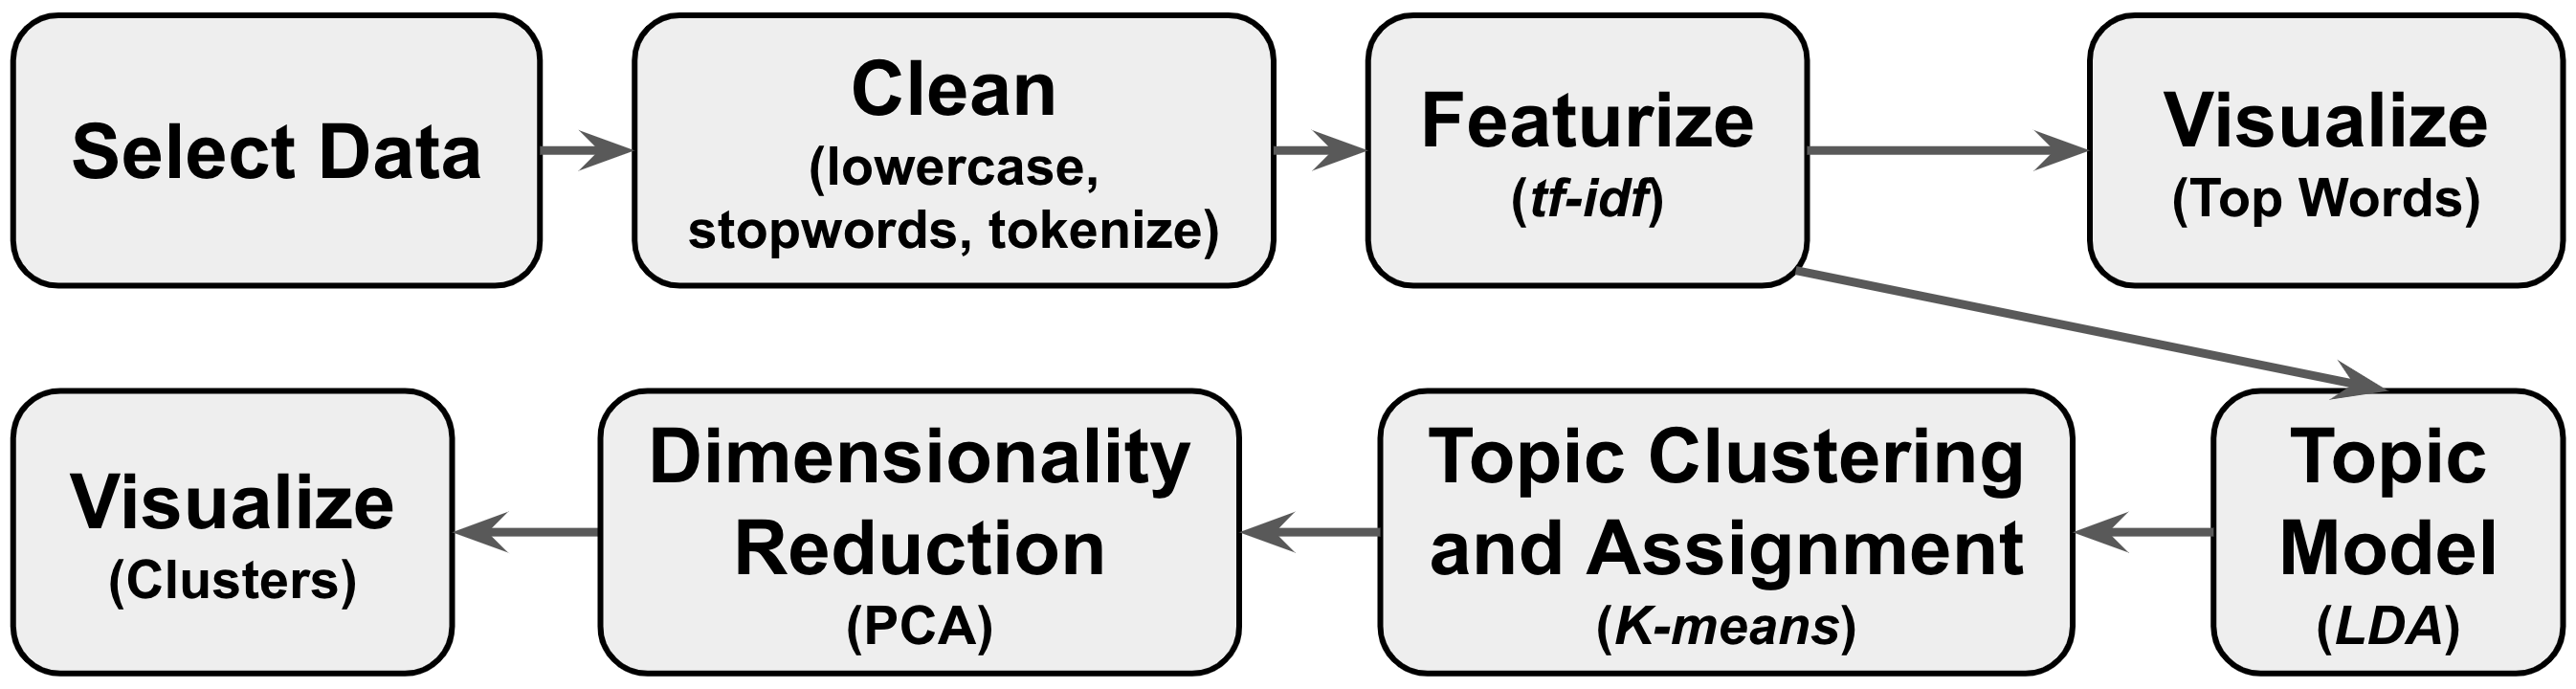
\includegraphics[width=\linewidth]{figures/workflow.png}
  \caption{\small An example \vita workflow for topic exploration. Even this basic workflow contains a diverse set of tasks. Interactive visualizations are useful across multiple stages in the workflow.\label{fig:workflow}} 
%   \vspace{-20pt}
\end{figure}

% \emtitle{C3. Data types and workflow diversity.} \vita workflows deal with heterogeneous data (\eg text, visualizations) and workflows (\eg in use-cases like text summarization, sentiment analysis). While there are a number of \vita tools for specific workflows~\cite{liu2018bridging}, more often than not these tools use a stack of independent solutions for data storage and
% processing glued together by scripting languages like Python and R.
% These bespoke solutions typically don’t support direct data manipulation and interactive visual coordination. As a result, users are often forced to develop new and heavily customized systems on top of these solutions.

\emtitle{C3. Arduous workflow authoring.} 
\vita workflows contain a variety of operations, \eg cleaning, featurization, interactive visualization, classification. Similar to relational~\cite{codd} or data visualization algebra~\cite{satyanarayan2016vega}, \vita operations with similar objectives can be grouped into high-level categories. Moreover, operations in different categories can be combined to compose new operation pipelines. For example, cleaning and featurization can be combined into a preprocessing pipeline. As existing systems lack any formalization of the operations and their application, the onus is on the user to design the optimal analytics workflow for different use-cases.

% \emtitle{C5. \vita Session management.} As demonstrated in the usage example, \vita workflows warrant the trial-and-error style  iterative approach---users often need to reproduce previous steps of the workflow, make updates, and rerun the subsequent steps. 
% Therefore, ensuring reproducibility of  \vita sessions requires management of dataset versions produced by various operations, the operation logs, and different states of and interactions on the visual representations of the data. 
% Prior work from the data management community focused on versioning structured datasets~\cite{huang2017orpheusdb}, versioning code for debugging workflows~\cite{brachmannbyour,miao2016provdb} and managing deep learning models~\cite{miao2016modelhub}.
% However, these systems lack support for versioning an end-to-end \vita workflow involving heterogeneous data types and user interactions spanning multiple views. 





\section{Design Criteria} 
\label{sec:design}
We propose the following design principles to address the challenges related to \vita:

\emtitle{D1. In-situ analytics.}
\vita systems should provide a one-stop-shop (\textbf{C1}) where users can directly
manipulate (spreadsheets) and visualize (visualization tools) data while writing scripts (notebooks) to immediately view the effects on data and visualizations without context switching between tools.

\emtitle{D2. Multi-view coordination.}
Beyond integrating multiple views within a single interface, \vita systems should enable coordination between these views (\textbf{C2}).
Multiple coordinated views capture the context of the user's exploration across different views~\cite{wang2000guidelines} and help users understand the data better as they view it through different connected representations.

\emtitle{D3. Heterogeneous data management.}
\vita systems should support heterogeneous data types (\eg texts, visualization), treating them as first-class citizens of the underlying data model (\textbf{C3}). Instead of developing bespoke data management solutions, \vita systems should adapt their underlying storage model to
accommodate these data types and also enable a tight coupling between the data model and the analytical workflows to ensure fast and efficient data access.

\emtitle{D4. Expressivity and accessibility.}
\vita systems should provide an expressive specification language to represent and communicate the entire breadth of workflows within the domain (\textbf{C4}). 
%The specification language should characterize the data domain with heterogeneous data types, abstract operations into high level categories, define rules for synthesizing new operations, and capture the coordinated interactions between multiple views. 
Moreover, the specification language should be accessible to existing tools to allow more expressive operations. 
For example, the specification language can be packaged as a Python library with an interactive widget with support for a subset of \vita operations in a computational notebook.

\emtitle{D5. Provenance.}
\vita systems should support advanced provenance tracking for heterogeneous data types and various workflows to ensure reproducibility and encourage workflow and data re-use. 
Moreover, these systems should track user interactions on visual components to enable versioning of states of and dependencies among different views.





\section{Visual Text Analysis Using \system}
\label{sec:system}
We now discuss various components of \system user interface and explain how these components enable users to perform various text data analysis and visualization tasks. The three key components of the interface are a Data View, a Chart View, and a Code Editor. \system also has a dropdown-style operations menu within it's menubar.
The operations menu allows users to use built-in text analysis and visualization operation. 

\stitle{Code Editor and Operations Menu.}
The Code Editor design (see Figure~\ref{fig:fe}C) is inspired by computational notebooks. 
However, the traditional notebooks are often criticised for their linear representation, making it difficult to explore visualizations and data and to maintain the context of the data analysis workflow~\cite{?}. The \system Code Editor only supports writing, editing, and executing scripts---visualizations and data tables are displayed separately in Chart View and Data View, respectively. The multi-view representation is intended to help users in more flexible exploration within the analytics session. Users can write scripts in the Code Editor in Python language. We also introduce a set of operators for analyzing and visualizing data using an algebra called \vta (discussed in Section~\ref{sec:vta}). The \vta commands are accesible via a Python library called \vital (also discussed in Section~\ref{sec:vta}).
Figure~\ref{fig:workflow} shows an example workflow written in \vital where a user first loads a review data, then cleans the ``review'' column within the dataset, featurizes the data, and finally, creates a bar chart visualization. We discuss how data and charts are generated and displayed in their corresponding views later.

\begin{figure}[!htb] 
%  \vspace{-10pt}
  \centering
  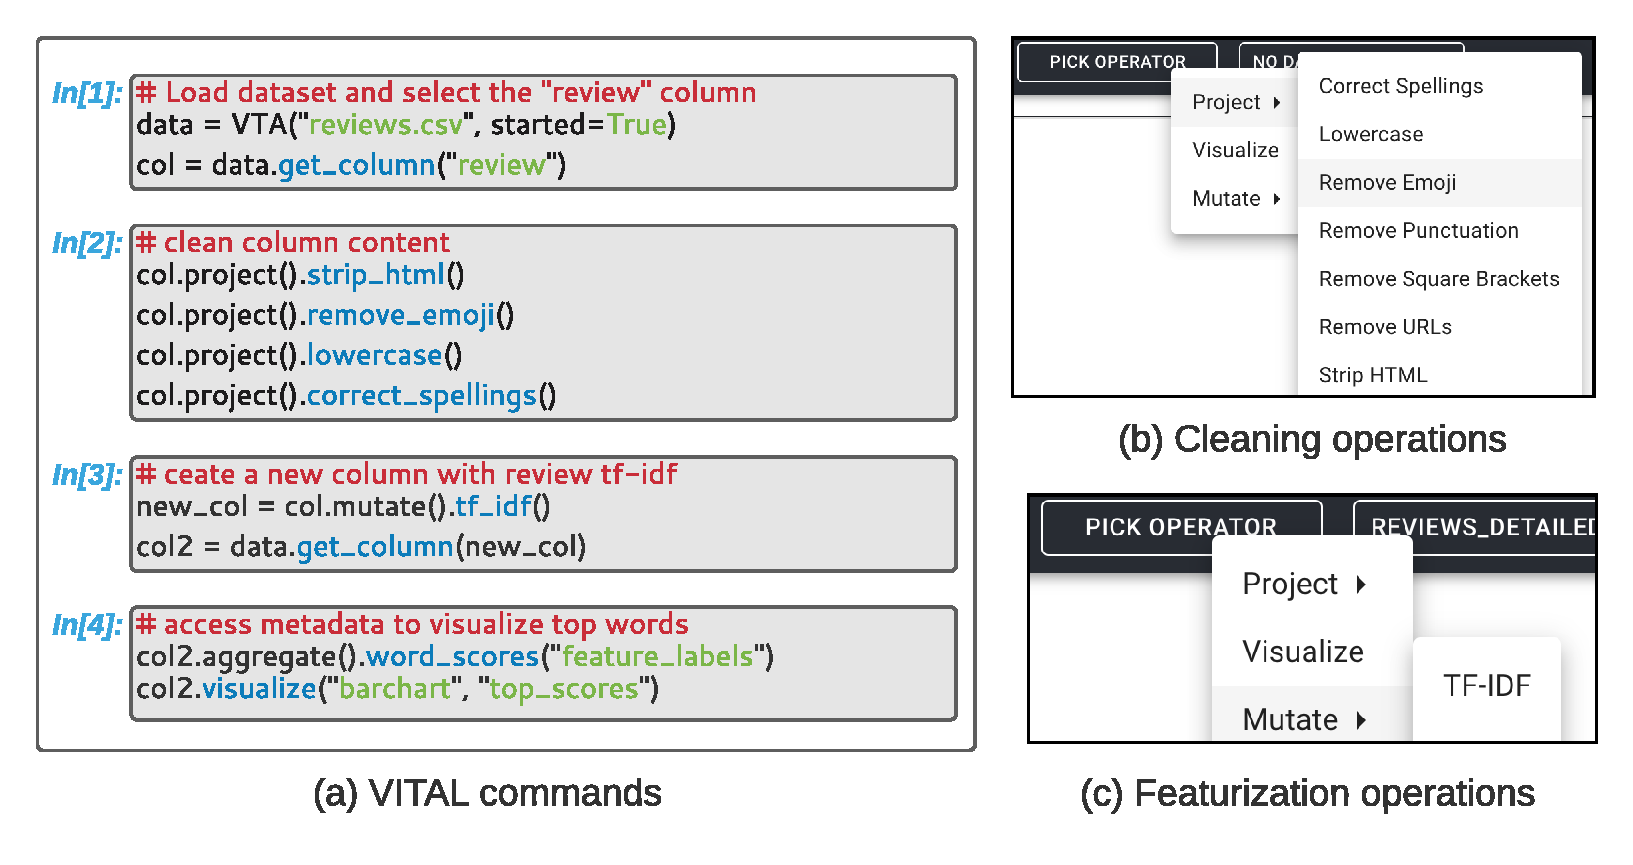
\includegraphics[width=\linewidth]{figures/vital.pdf}
  \caption{\small \system provides an API called \vital (visual interactive text analysis library) to enable users to run \vta operations within Notebook View. (a) An example usage of \vital. A user first loads a review data, then cleans the ``review'' column within the dataset, featurizes the data, and finally, creates a bar chart visualization. Instead of writing scripts, the user can also utilize the built-in (b) cleaning, (c) featurization, and visualization operations available via the drop-down menu. The \vital equivalences of the menu-driven operations are also interactively prompted to the user in Notebook View for improved accessibility and reuse. \label{fig:workflow}} 
  %\vspace{-20pt}
\end{figure}

Instead of writing \vital commands, users can also utilize the Operations Menu to execute built-in relevant analysis and visualization operations (see Figure~\ref{fig:workflow}a, ~\ref{fig:workflow}b, and ~\ref{fig:workflow}c). Other features in the Operations Menu involve uploading data and pre-trained models. However, the Code Editor provides more flexibility and a wider range of operations. For example, users cannot create custom operators from Operations Menu. The Code Editor supports these features. We show in Section~\ref{sec:vta} how users can write custom functions in Code Editor that become new operators in Operations Menu. 

\todo{Operations menu is interaction is added to Code Editor. Any metadata created becomes part of the operator view suggestion.}


\begin{figure}[!htb] 
%  \vspace{-10pt}
  \centering
  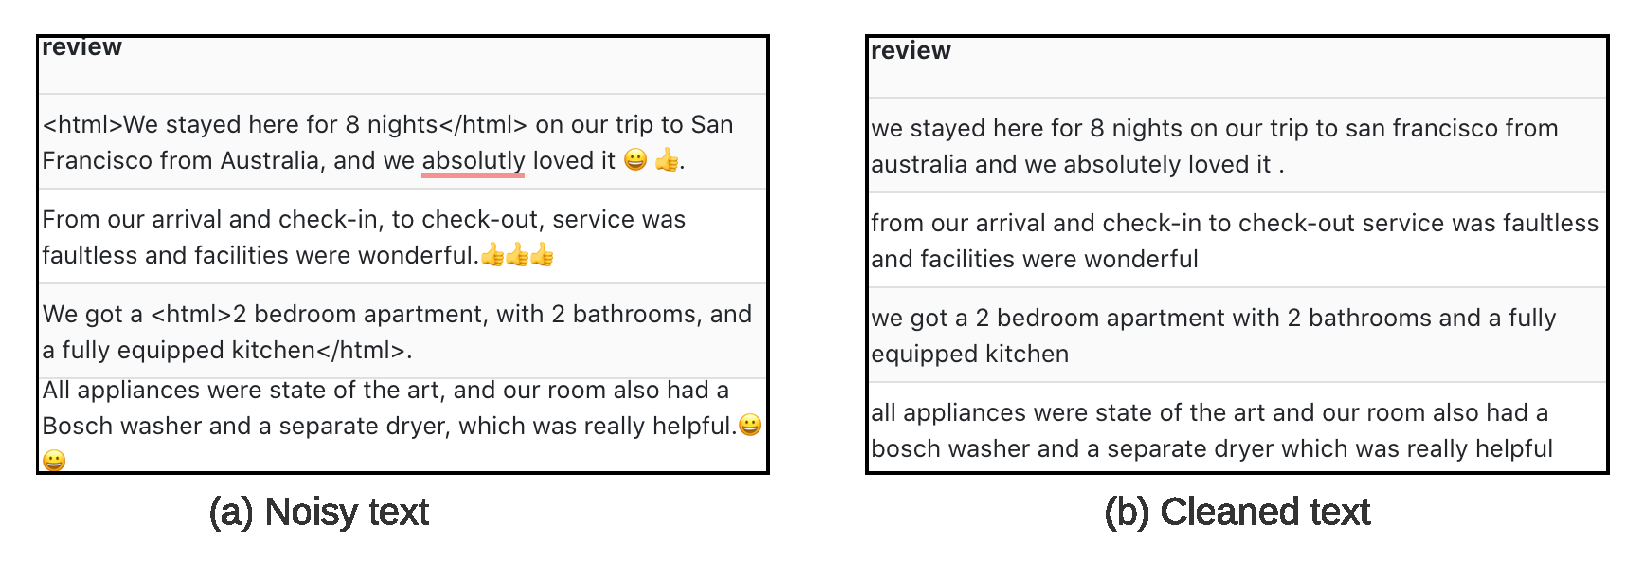
\includegraphics[width=\linewidth]{figures/data_view_clean.pdf}
  \caption{\small \system dynamically updates the effects of operations---run either via the interactive menu or from Notebook View---across relevant views of the data. (a) Noisy data with HTML tags, emojis, and typos in the ``review'' column. (b) After a user performs various cleaning operations on the `review'' column as shown in Figure~\ref{fig:workflow}, the changed column data is immediately displayed in Data View. \label{fig:dataview}} 
  %\vspace{-20pt}
\end{figure}

\stitle{Data View.}
Data View (see Figure~\ref{fig:fe}C) shows a tabular representation of the underlying data. Note that the underlying data structure in \system is a dataframe~\cite{rahman2020leam}. Data View is kept in sync with the dataframe---any changes made to the dataframe is immediately reflected in Data View. For example, in Figure~\ref{fig:dataview} when a user cleans the review column in the dataframe, the corresponding cleaned data is displayed in the Data View. Tehrefore, changes to the underlying data is immediately visible to the user. In traditional script-based systems like computation notebooks, users are required to explicitly specify a print operation to view and inspect data. \system currently supports one dataset per session. Whenever a new dataset is uploaded, the Data View is refreshed to display the new dataframe corresponding to that dataset. We discuss how to explore multiple datasets in Data View in Section~\ref{sec:discussion}. 
\todo{Future work, support filtering data in Table View which will create a new filtered the dataframe and pickle the original dataframe. Support multiple datasets.}

\stitle{Chart View.}
Text data analysis often involves generating visualizations like data distribution, aggregated summaries of attributes, to obtain further insights.
\system enables users to generate visualizations either from the Code Editor or Operations Menu and displays those visualizations in the Chart View. The charts are displayed within a carousel (see Figure~\ref{fig:fe}B). We create the visualizations using Vega-Lite~\cite{satyanarayan2016vega}. Figure~\ref{fig:chartview_interact}a shows a barchart corresponding to the \vital command in the fourth cell of the Code Editor in Figure~\ref{fig:workflow}a.

\todo{Fig 5 (a) is a bit confusing. It reads as if when a bar chart visualization is created, an arbitrary selection is also created and displayed by default.} 

\begin{figure}[!htb] 
%  \vspace{-10pt}
  \centering
  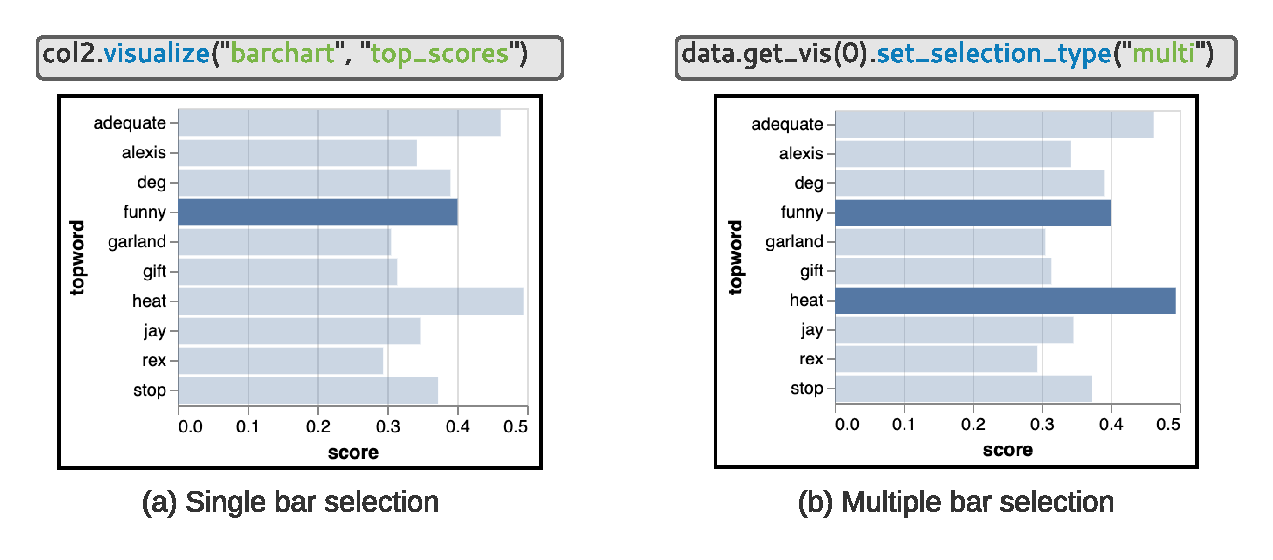
\includegraphics[width=\linewidth]{figures/chart_view_interact.pdf}
  \caption{\small \system enables a user to declaratively specify interactive selection (i.e. programmatic  mouse `clicking' or `brushing' effects) and view coordination. (a) A bar chart of top words in reviews ranked by their TF-IDF scores. The default selection  behavior is to select a single bar. (b) The user  dynamically specifies the \code{multi} selection type 
  to select multiple bars. We show the corresponding \vital command above each chart. \label{fig:chartview_interact}} 
  %\vspace{-20pt}
\end{figure}

However, Vega-Lite requires users to specify the visual encoding as well as supported interactions (\eg single or multple bar selection) before chart generation. \system enables users to specify such interactions dynamically using \vta view coordination algebra, \ie new interactions can be added on the fly even after the visualizations are created. For example, as shown in Figure~\ref{fig:chartview_interact}b, users can update the selection type of the barchart in Figure~\ref{fig:chartview_interact}a to enable multiple bar selection. Moreover, using the coordination algebra, users can also dynamically specify external coordinations between Data View and charts within the Chart View (see Section~\ref{sec:vta}). Vega-Lite currently does not provide a formal interaction grammar for external coordination. One alternative is to leverage the Vega Signals API~\cite{satyanarayan2015reactive} to enable coordination of Vega-Lite charts with external views.
However, unlike \system users cannot specify such coordination dynamically. For example, Figure~\ref{fig:chartview_coordinate} shows how users can enable coordination between the barchart, and scatterplots. Such dynamicity allows users to augment the visualizations instead of recreating charts and connect different views on demand to investigate data relationships. 

\begin{figure}[!htb] 
%  \vspace{-10pt}
  \centering
  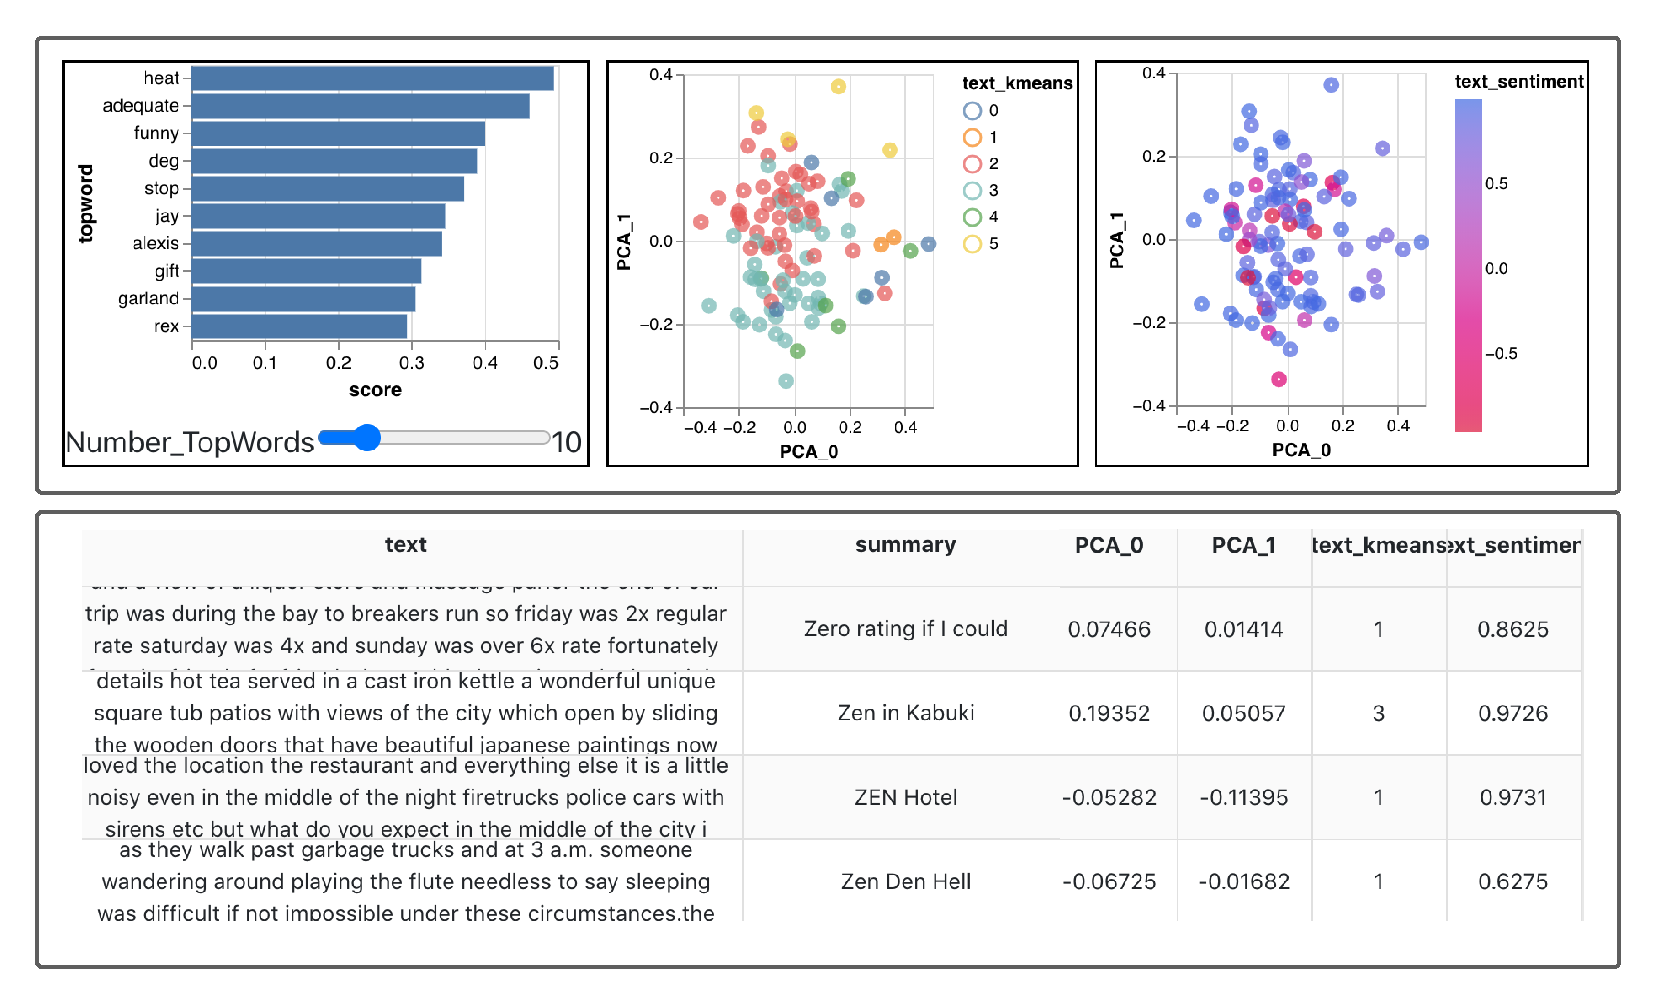
\includegraphics[width=\linewidth]{figures/chart_view.pdf}
  \caption{\small \todo{Draw figures} Example of dynamic coordination creation. The figure displays the barchart (generated in Figure~\ref{fig:chartview_interact}), a Scatterplot of reviews clustered using $k$-means clustering, and the corresponding data in Data View. To relate a word in the chart with reviews both in Data View and the scatterplot, the user issues a \vital command in Code Editor (see inset). Clicking a bar in the barchart filters reviews in Data View and highlights relevant reviews in the scatterplot. \label{fig:chartview_coordinate}} 
  %\vspace{-20pt}
\end{figure}








\section{Visual Text Algebra and the \vital API}
\label{sec:vta}
\system leverages an algebra for visualization and analysis of text dataset, \vta~\cite{rahman2020leam}.
We further enrich \vta by adding a number of operators in \system related to data preprocessing, model building, and visual coordination. \system also provides an API called \vital---developed as a python library (visual interactive text analysis library)---that enables users to write \vta commands in the built-in computational notebook. We now briefly introduce \vta and then demonstrate the corresponding specification library \vital that we have developed.

%To the best of our knowledge, an algebra for \vita has never
% been defined previously. 
%However, our work draws inspiration from relational algebra~\cite{codd} and prior work on visualization grammars~\cite{satyanarayan2016vega,satyanarayan2015reactive,stolte2002polaris,bostock2009protovis,bostock2011d3}.

% \candidate{We now explain how users specify \vita workflows in \vta.
% While explaining the algebra, we also demonstrate how \vta captures various tasks in the usage example in Section~\ref{sec:example}
% (see Figure~\ref{fig:fe},~\ref{fig:use-case-a}, and~\ref{fig:use-case-b}). As shown in these figures, \vta operators can be specified in a \emph{json} format or as declarative commands that are available through a \vta library in Python.}
\subsection{Overview of \vta}
\vta supports various operators for selecting a subset of the data, transforming selected data into various representations for analysis, and coordinating different views within the interface. \vta operations are applied to the underlying dataframe in \system and charts within Chart View. The operators are classified into three four high level categories: selection, transformation, composition, and coordination~\cite{rahman2020leam}. We now briefly explain these operators.

\subsubsection{Selection operators.}
Selection operations sub-select data points from a given data which can be either the raw data in Data View or visualization mark(s) in Chart View. Supported selection types include a data point (single), a collection of data points (either a list or an interval). 
\vta leverages the Vega-Lite~\cite{satyanarayan2016vega} to support similar types of selections on visualizations. Figure~\ref{fig:chartview_interact}b shows an example of single point selection on a barchart. On the other hand, as shown in Figure~\ref{fig:chartview_coordinate}, highlighting multiple points in the scatteroplot or filtering rows in the table are examples of multiple point selection.

\subsubsection{Transformation operators.}
A transformation operator changes the actual data. For example, cleaning operation remove noisy elements (\eg HTML tags, emojis, punctuations) while featurization operators create vector representation of texts.
The transformation operation has five subclasses~\cite{rahman2020leam}: \code{project}, \code{mutate}, \code{aggregate}, \code{set}, and \code{visualize}. We introduce a number of new operations in \system for each operator class. Table~\ref{tab:operators} shows a snapshot of the operators supported by \system. The bold operators are new operations supported by \system. According to Rahman et al.~\cite{rahman2020leam}, (a) the \code{project} operators change the dimensionality or cardinality, or update the content of data, (b) the \code{mutate} operators transform data into a different data type, (c) the \code{aggregate} operators compute aggregated summary of the input data, (d) the \code{set} operators support set operations, and the \code{visualize} operator generates visualizations of data. 

\begin{table}[]\scriptsize
\caption{Examples of \vta operators.}
\begin{tabular}{ccl}
\textbf{Class} & \textbf{Operator} & \textbf{Example} \\ \hline
  Selection    &     selection     &  \textit{select}, \textit{filter}       \\ \hline
            &     project     &   \textit{lowercase, remove\_punctuation,} \\ 
            & & \textit{remove\_stopwords, PCA,}       \\
            & & \textbf{\textit{remove\_emoji, strip\_html,}} \\
            & & \textbf{\textit{remove\_url, correct\_spellings}}\\
    Transformation            &     mutate     &   \textit{tokenize, tf\_idf, $k$-means,} \\ 
               & & \textit{get\_sentiment}, \textbf{\textit{predict}}      \\
                &     aggregate & \textit{\textbf{count\_tokens}}, \textit{word\_scores}        \\
                &     set &  \textit{get\_unique\_values}       \\
                &     visualize     &    \textit{barchart (horizontal, vertical, \textbf{stacked}),}\\
                & &  \textit{scatterplot, \textbf{heatmap, line chart}}     \\ \hline
                &     combine     &  \textit{combine}       \\
    Composition            &     synthesize     &   \textit{synthseize}      \\
                &     udf     &    \textit{\textbf{add, apply}}     \\ \hline
       Coordination      &    internal      &  \textit{\textbf{set\_selection\_type}}       \\
        &     external     &  \textit{\textbf{uni\_link, bi\_link}}       \\ \hline
\end{tabular}
\label{tab:operators}
\end{table}

As shown in Table~\ref{tab:operators}, we have added a number of new data cleaning operators (\code{project}) while adding new visualizations and visual coordinations.
We have enhanced the scope of \code{mutate} operators by allowing users to upload pre-trained models perform operations like classification, regression. For example, users can access an uploaded model using the \code{get\_model} command and then use the \code{predict()} operation to perform classification.

\subsubsection{Composition operators.}
Users can combine multiple existing operators to create customized operators. Two such operators introduced by Rahman et al.~\cite{rahman2020leam} are \code{combine} and \code{synthesize}. In \system, we enable users to compose user defined functions and add those as new operators (see Table~\ref{tab:operators}). For example, as shown in Figure~\ref{fig:udf}, user creates a new function to generate top $n$-grams in a given corpus, for example, a set of reviews and then uses \vital to load and then apply the UDF.

\begin{figure}[!htb] 
%  \vspace{-10pt}
  \centering
  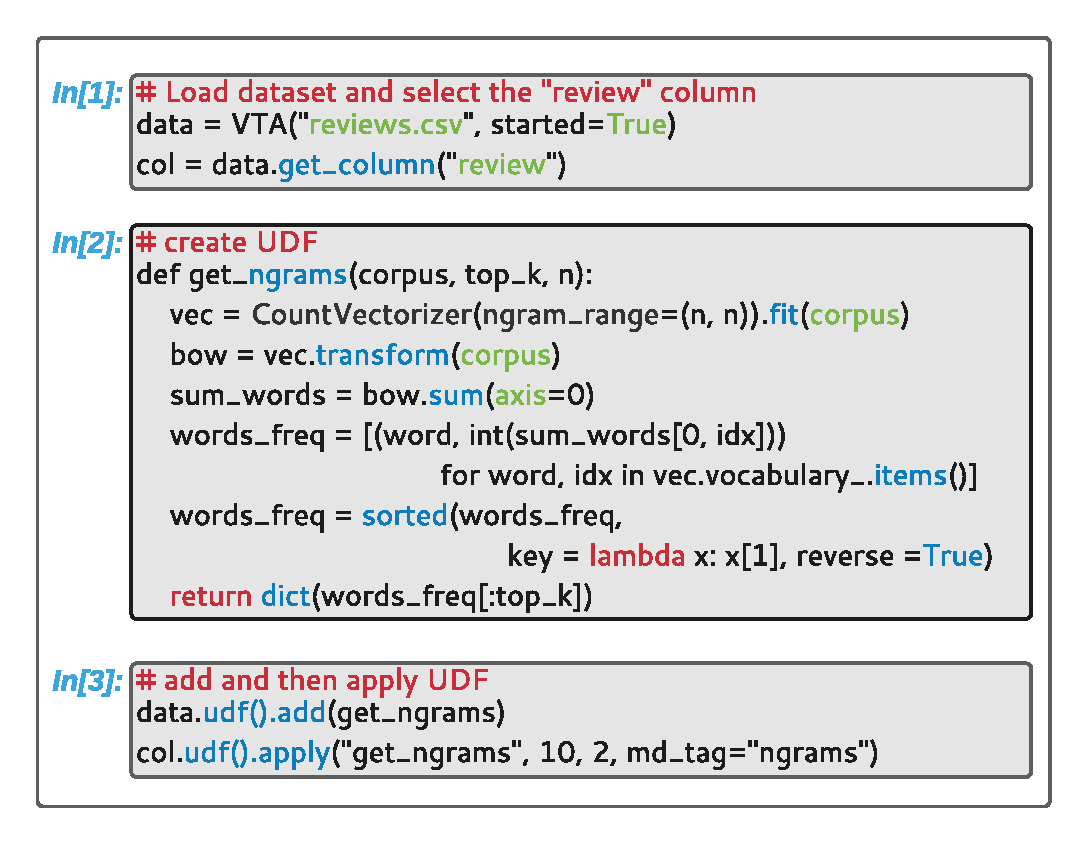
\includegraphics[width=\linewidth]{figures/udfs.pdf}
  \caption{\small  Example of adding a user-defined function (UDF) as a new operator and then applying the operator. The example UDF here computes the top $K$ $n$-grams of a given corpus. In general, \system enables users to create new operators by either composing (`piping') existing operators or specifying custom functions (UDFs).\label{fig:udf}} 
  %\vspace{-20pt}
\end{figure}



\subsubsection{Coordination operators}
The coordination operators in \vta are designed to enable coordination among views. We have enhanced the existing \vta implementation~\cite{rahman2020leam} so that users can dynamically add interactions to Data View and charts in Chart View. As show in Table~\ref{tab:operators}, there are two types of coordination operators: \code{internal} and \code{external}. The \code{internal} coordination operators allow users to set the selection type of an existing visualization---for example, setting the barchart selection from \emph{single} to \emph{multi} in Figure~\ref{fig:chartview_interact}. The \code{external} coordination operators allow users to enable coordination among views in \system. While the initial implementation of \vta supports only unidirectional coordination~\cite{rahman2020leam} (\emph{uni\_link} in Table~\ref{tab:operators}), \system supports bidirectional coordination using the \emph{bi\_link} operation. Once two views are linked by a bidirectional coordination, interacting with one visualization will update/modify the other visualization. For example, in Figure~\ref{fig:chartview_coordinate}, the barchart and scatterplot are linked via a bidirectional coordination. Therefore, selection a visualization mark (\ie bar or circle) in either updates the corresponding visualization. Moreover, \system also supports coordination of more than two views~\cite{rahman2020leam}. For example, adding a coordination between the barchart and Data View automatically links the scatterplot with the Data View (Figure~\ref{fig:chartview_coordinate_multi}). \system maintains a coordination graph to keep track of the linked views which we discuss in Section~\ref{sec:system}.

\begin{figure}[!htb] 
%  \vspace{-10pt}
  \centering
  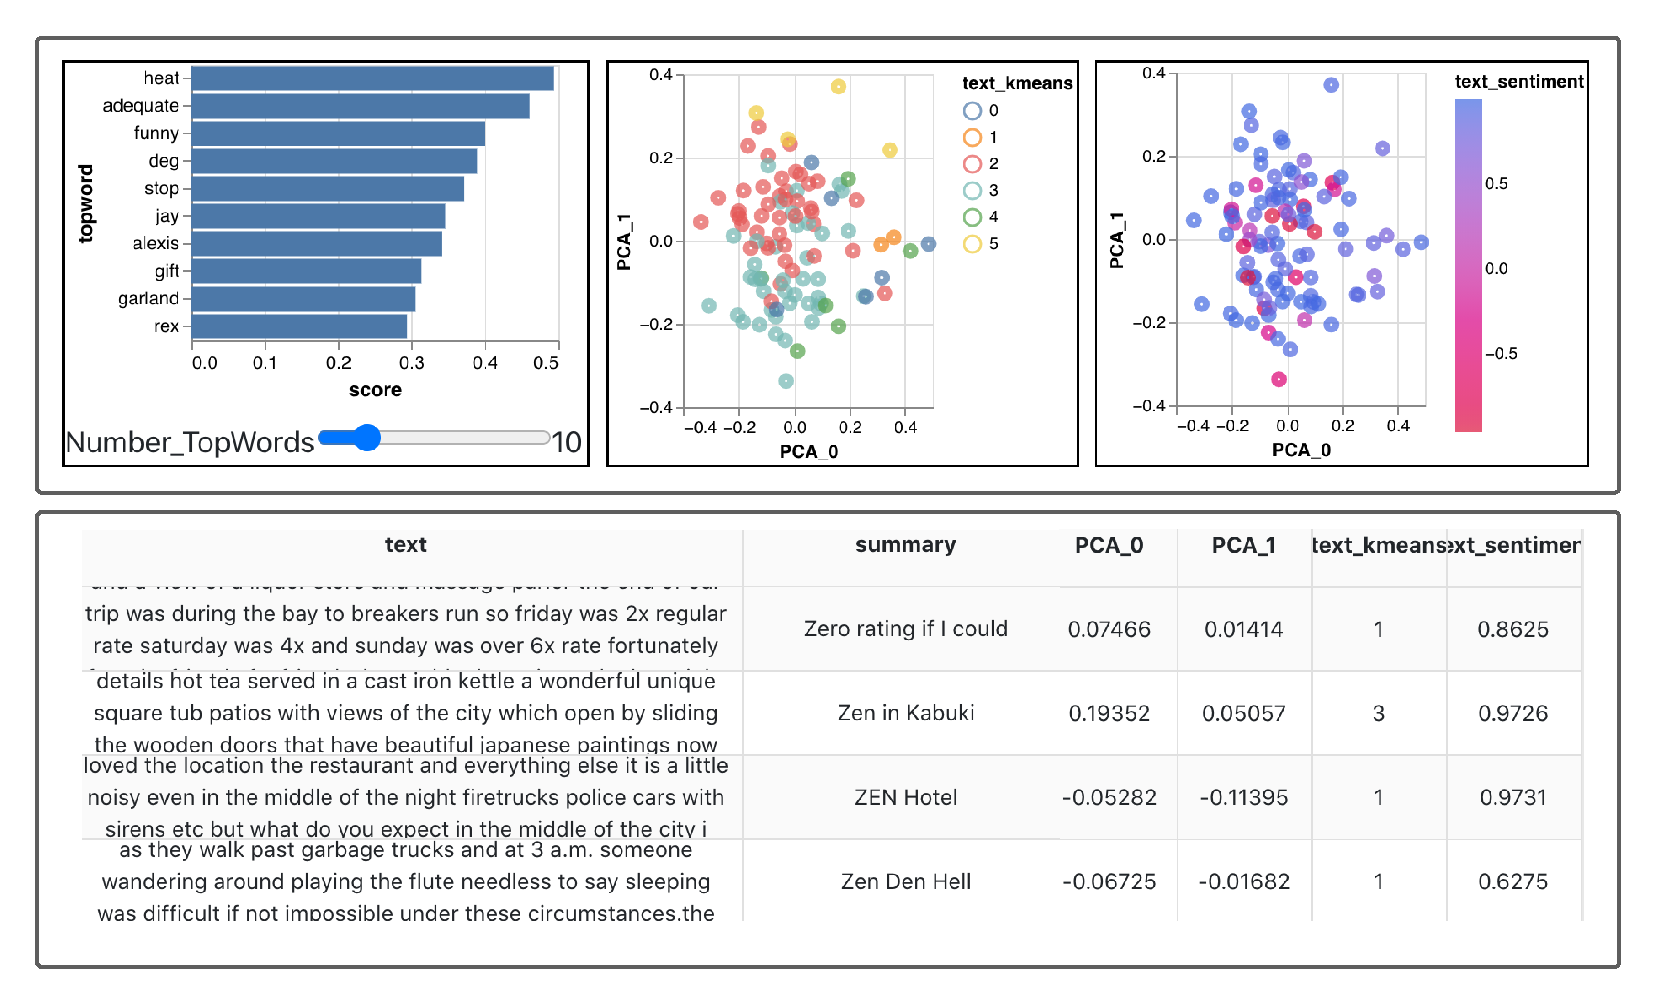
\includegraphics[width=\linewidth]{figures/chart_view.pdf}
  \caption{\small \todo{Draw figures} Example of dynamic coordination creation. The figure displays the barchart (generated in Figure~\ref{fig:chartview_interact}), a Scatterplot of reviews clustered using $k$-means clustering, and the corresponding data in Data View. To relate a word in the chart with reviews both in Data View and the scatterplot, the user issues a \vital command in Code Editor (see inset). Clicking a bar in the barchart filters reviews in Data View and highlights relevant reviews in the scatterplot. \label{fig:chartview_coordinate_multi}} 
  %\vspace{-20pt}
\end{figure}


\subsection{\vital: Declarative \vta Specification}
The JSON-style specifications for \vta introduced by Rahman et al.~\cite{rahman2020leam} can be difficult for the users to compose with advanced operations requiring multiple nested objects. Moreover, such specification format is quite different from popular scripting languages like R and Python that are widely used by analysts. Therefore, we have developed \vital, a python-based library for declaratively specifying \vta commands in Code Editor of \system. We show several examples of \vital commands that implement the \vta operators in Figure~\ref{fig:workflow} (\code{project}, \code{mutate}, \code{visualize}, \code{aggregate}), Figure~\ref{fig:chartview_interact} (\code{visualize}, \code{coordinate}), and Figure~\ref{fig:udf} (\code{udf}. All four \vta operator classes are packaged as a \code{VTA} class. To enable \vta operators on a dataset, users are required to instantiate a \code{VTA} object in Code Editor (see the first cell in Figure~\ref{fig:workflow} and~\ref{fig:udf}). The \vital commands are compiled and executed by the backend python runtime. \system employs a \emph{task queue} to manage the sequence of \vital commands written in the Code Editor (see Section~\ref{sec:system}). 


\section{\system Architecture}
\system is developed as a web application and is implemented using ReactJS and Flask framework. We now discuss the system architecture in detail. 
\begin{figure}[!htb] 
%  \vspace{-10pt}
  \centering
  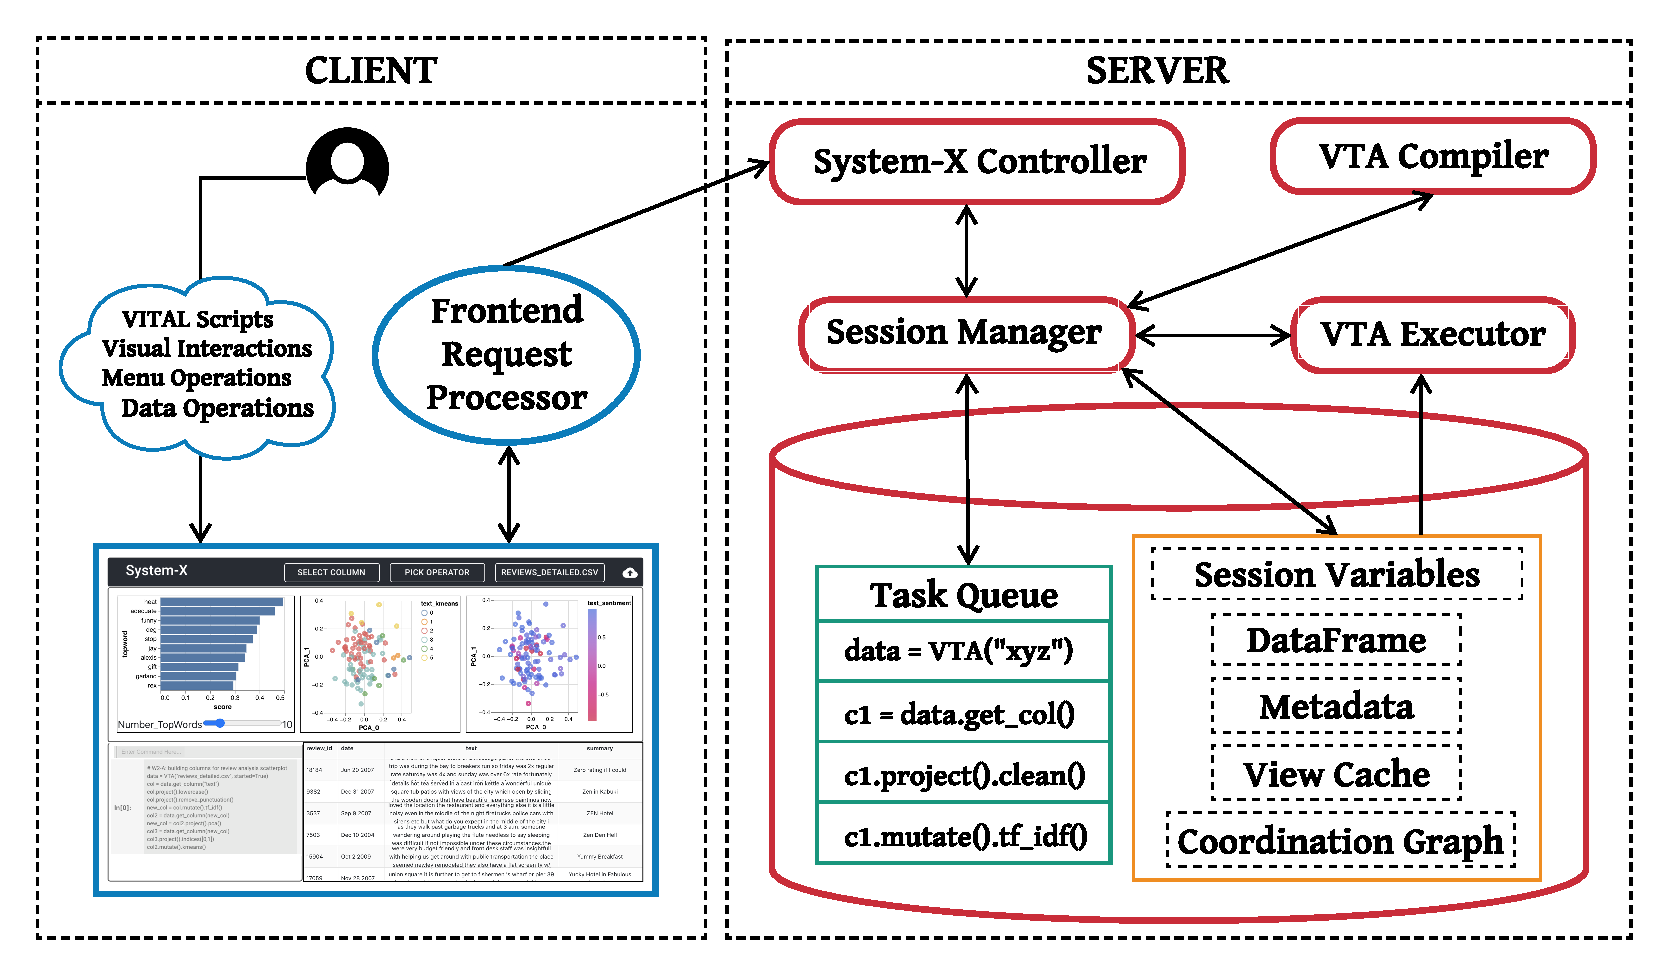
\includegraphics[width=\linewidth]{figures/leam_arch.pdf}
  \caption{\small \system architecture.\todo{Repeat the most important architectural design goals.} \label{fig:arch}} 
  %\vspace{-20pt}
\end{figure}


We depict the architecture
diagram in Figure~\ref{fig:arch}.
On the client or front end side,
the \system client is responsible
for capturing user input 
on various interface components,
and for rendering the views
based on results returned by the
back-end. Examples of user interactions include
\vital commands in Code Editor, 
operator selection in Operations Menu operator,
interaction with Data View and charts in Chart View.
Given any user interaction
on the front end,
the \system Request Processor
issues a request to the backend \system Controller.
This controller manages the uploaded data and sessions
while propagating user interactions to the {\em session
manager}. 

The session manager interprets the user 
interaction---any interactions on the Operations Menu
is sent to a lightweight \vta Compiler~\cite{rahman2020leam}
while the \vital commands on the Code Editor are pushed in a task queue.
The \vta compiler translates the user-selected operator to a \vital
command which is then executed by the \vta Executor. 
Since users can either write single- or multi-line \vital commands,
\system backend employs a Task Queue to keep track of the sequence of
tasks. Whenever the \vta executor completes the execution of a \vital command, the session 
manager fetches an unprocessed command from the task queue and sends that to the
executor. The \vta executor leverages the python runtime to access any global or local variables in the session and executes the command on the desired data.

\system backend utilizes a customized dataframe called \vitaframe for enabling text data analysis~\cite{rahman2020leam} operations. \vitaframe columns are complex objects that not only contains the raw data, but also the schema of the column, associated metadata and the metadata schema type. For example,
in Figure~\ref{fig:workflow}a, in the third cell of the Code Editor, the user computes the \code{tf\_idf} feature vector of the review column, and adds the vector as a new column. As a byproduct of this operation, a dictionary of unique words called ``feature\_label'' is created which is a metadata of the newly created column. The dictionary metadat is later utilized to create a bar chart of top ranked words (Figure~\ref{fig:workflow}a fourth cell).
Such a column specification with schema is necessary to validate a \vta operation. \system session manger also employs a View Cache to track states of the front end components and always remains in sync with the front end. If the states of a component is updated after a \vital command execution, the changes are propagated to the front end. Also, \system employs a Coordination Graph to manage coordination among linked views. For each view in the front end, \system maintains an adjacency list---for any interaction on a view, all the views in its adjacency list are updated. For example, selecting a bar in the barchart in Figure~\ref{fig:chartview_coordinate_multi} updates the scatterplot and Data View in its adjacency list.




%\section{Usage Examples}\label{sec:usage}
\todo{Pick two Kaggle examples and show how \system implements those.}

\stitle{Tweet analysis.} Notebook workflow does exploratory analysis by visualizing parts of the initial dataset using different barchart/histogram visualizations. They do data cleaning and then create a model using GloVe for vectorization and keras for building the model. The model is a classifier that determines whether the tweet is a disaster or not.

\stitle{Spam detection.} Notebook workflow does initial exploratory analysis, cleaning/pre-processing, building the model, and then doing a visualization of the resulting confusion matrix as a heatmap. The SMS Spam Collection contains one set of SMS messages in English of 5,574 messages, tagged according being ham (legitimate) or spam. This corpus has been collected from free or free for research sources from the Internet. The aim to correctly predict a given piece of text as Spam or Ham.


% \begin{figure*}[!htb]
% \centering
% \begin{tabular}{ c c c}
%   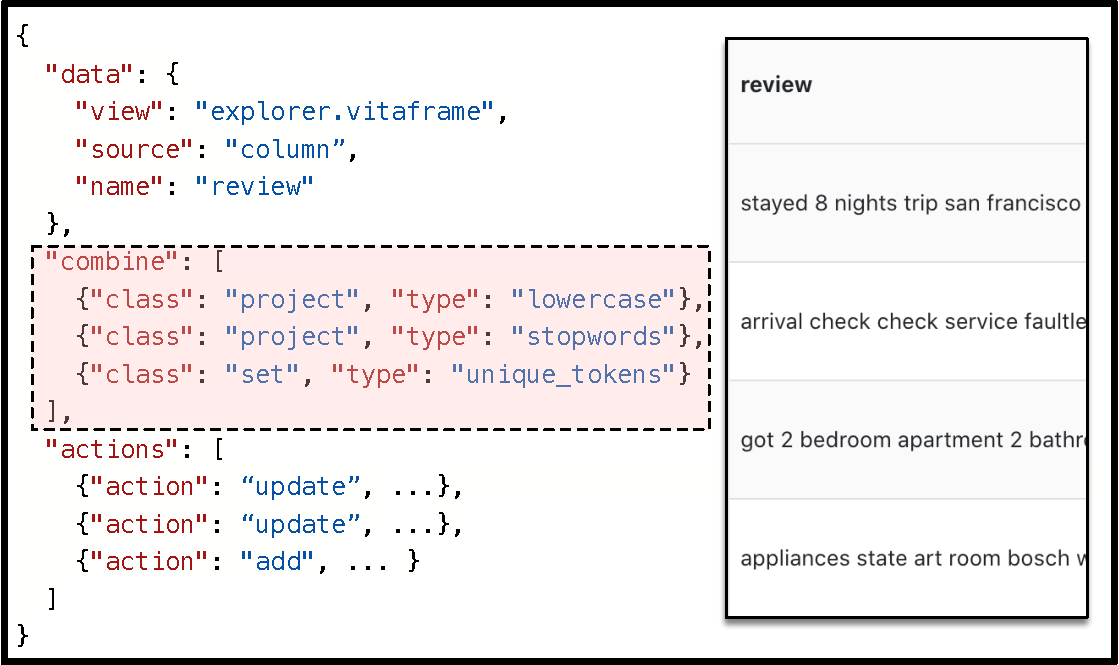
\includegraphics[width=0.3\linewidth,height=0.18\linewidth]{figures/combine_clean.pdf}   & 
%   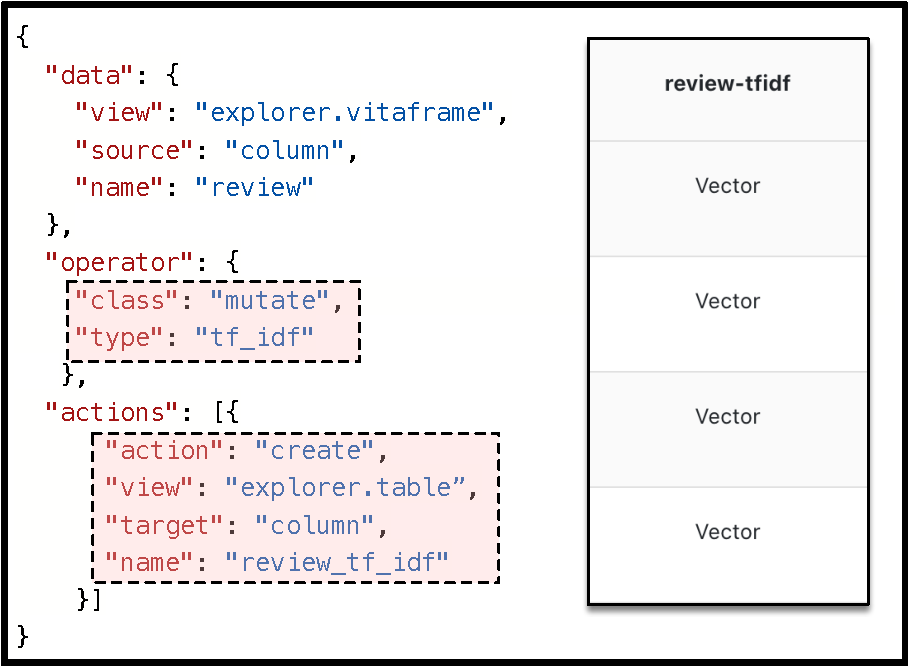
\includegraphics[width=0.3\linewidth,height=0.18\linewidth]{figures/tf_idf.pdf} & 
%   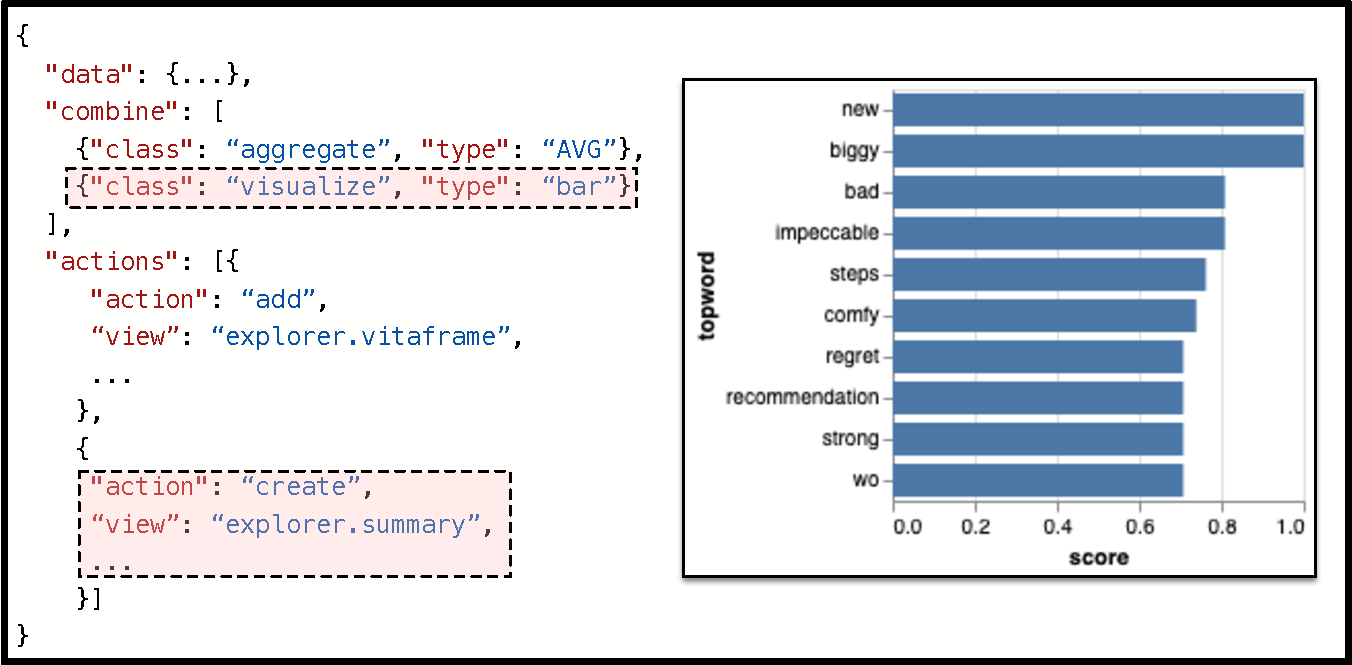
\includegraphics[width=0.3\linewidth,height=0.18\linewidth]{figures/barchart.pdf} \\
%      (a) Clean and generate metadata & 
%      (b) Create TF-IDF feature vector &
%      (c) Visualize top-words by TF-IDF score
% \end{tabular}
%     \caption{Example of \vta specification. (a) Use \emph{Combine} operator to clean data (\eg \emph{lowercasing}, \emph{stopwords removal}) and generate metadata (\eg \emph{unique\_token} to create token dicitionary) for use in subsequent steps. (b) Define featurization operation and subsequent action, \ie column creation in table view. (c) Compute average TF-IDF score of each token in the dictionary using \emph{aggregate} operator and then create barchart of top-ranked words using \emph{visualize} operator.}
% \vspace{-15pt}
%     \label{fig:use-case-a}
% \end{figure*}

% \begin{figure*}[tbp]
% \centering
% \small
% \begin{tabular}{ c c}
%   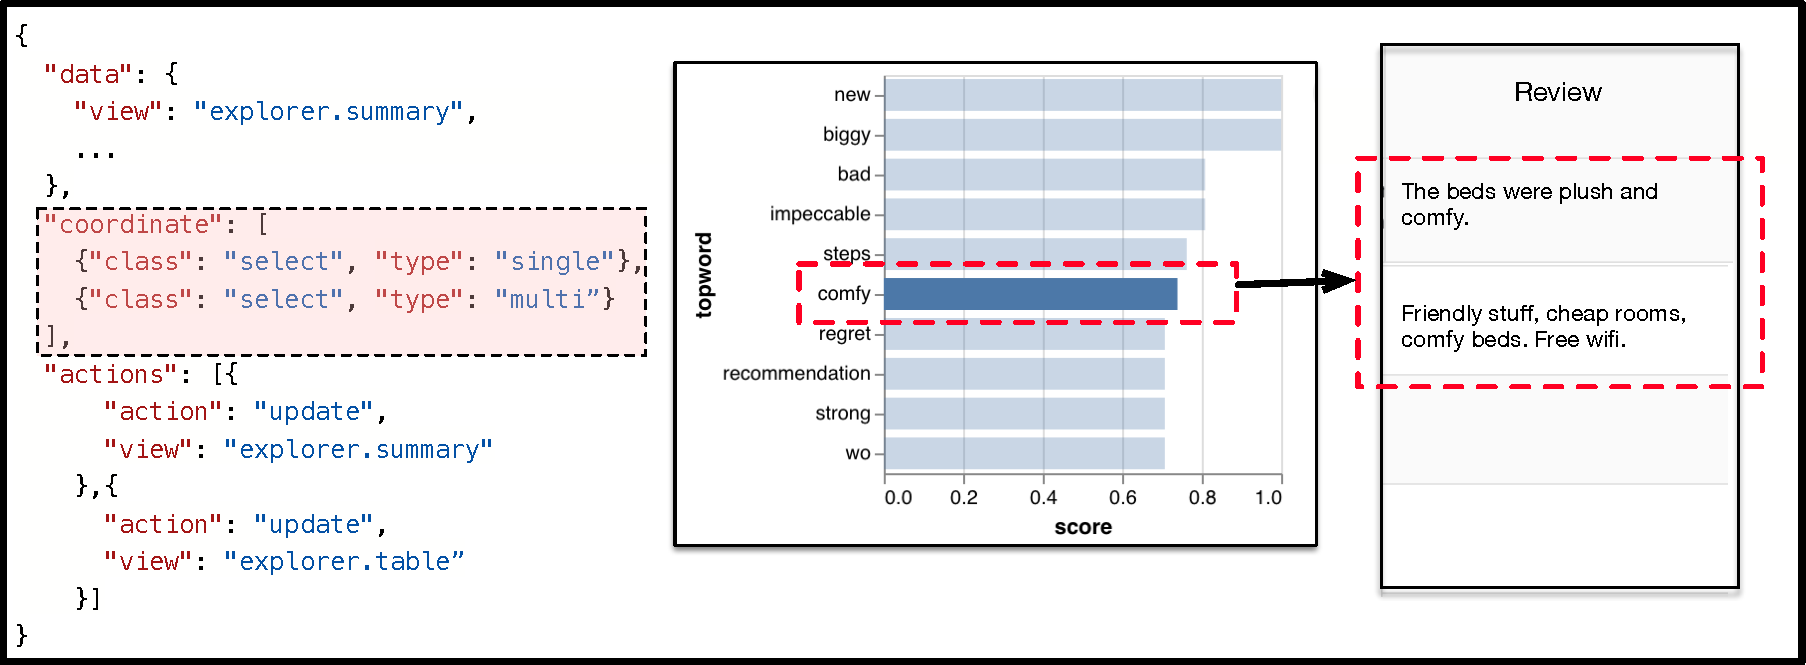
\includegraphics[width=0.5\linewidth,height=0.18\linewidth]{figures/unidirect_bar_table.pdf}   & 
%   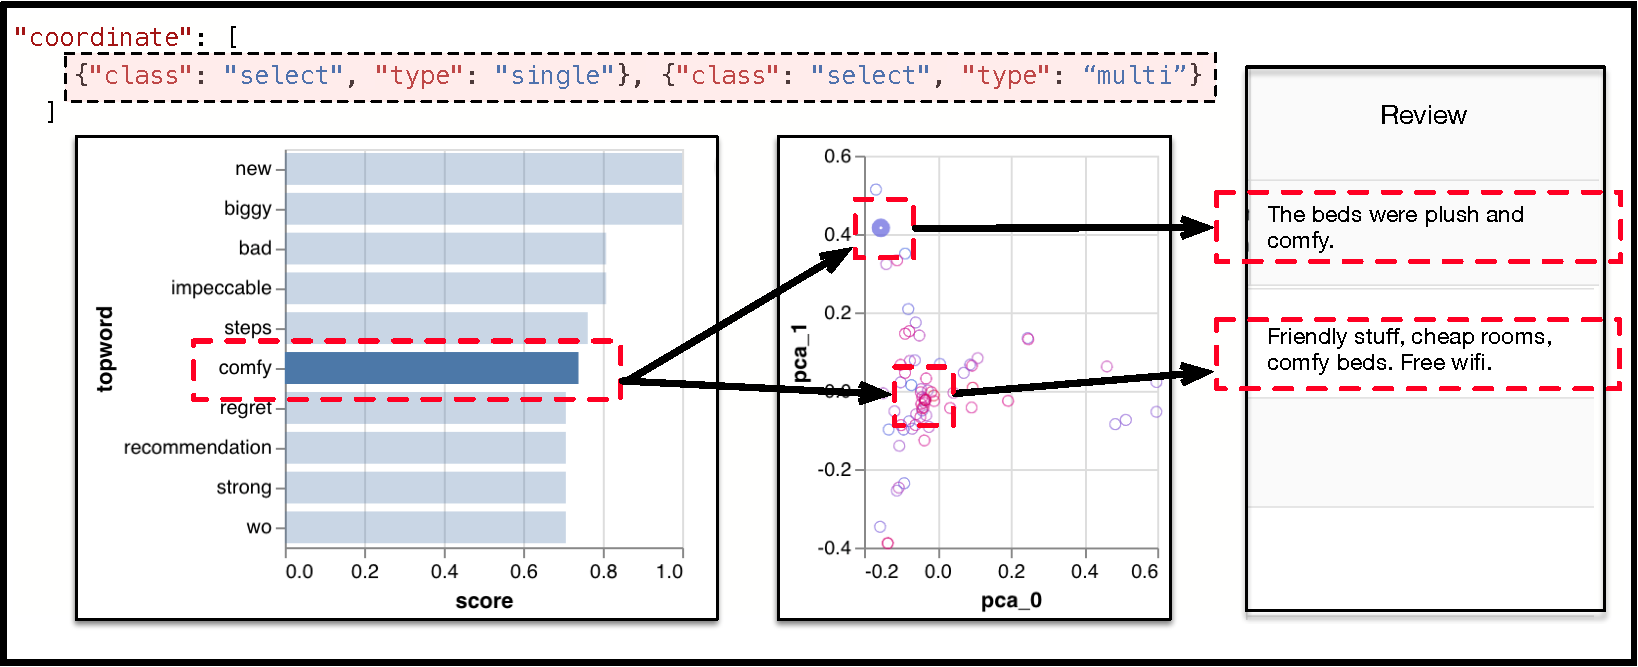
\includegraphics[width=0.5\linewidth,height=0.18\linewidth]{figures/unidirect_bar_table_scatter.pdf} \\
%      (a) Coordination of two views & 
%      (b) Coordination of three views 
% \end{tabular}
%     \caption{\small Multi-view coordination. (a) Use the \code{coordinate} operator to link the bar chart and Table View. Selecting a bar (word) in the bar chart triggers a \code{filter} by the selected word on Table View . (b) Coordinating the bar chart and scatterplot links the three views. Selecting a bar in the bar chart highlights relevant points in the scatterplot, and filters relevant rows in Table View.}
%     \label{fig:use-case-b}
%     \vspace{-15pt}
% \end{figure*}


\section{Observational Study Design}
\label{sec:study}
In this section, we present the design of an observational study
aimed at understanding the impact of \system in performing visual text analysis. 
Since there is no equivalent system for comparison, 
we studied how potential users of \system, for example, data scientists, would utilize various features and identified their pros and cons. 
We selected two text data analysis workflows 
from Kaggle that the participants implemented in
\system. Similar use-case driven evaluation have been performed for 
evaluating various interactive data analytics tools~\cite{fisher2012trust,moritz2017trust}. 
Our study was designed to answer the following questions:
\begin{itemize}
    \item[\textbf{RQ1}] How did \system and its components affect participants' experience at various steps within their text analysis workflow?
    \item[\textbf{RQ2}] How did participants employ to various \system features within their analytics pipleline, \eg direct data manipulation, built-in operators, notebook commands, view coordination, and in-situ visualization. 
\end{itemize}

\subsection{Participants}
\label{sec:participants}
To ensure that prior experience with text data analysis 
didn't affect the performance of participants during the tasks, 
we recruited two participants at \company with extensive experience in model building, hypothesis testing, and insight exploration with text data. One of the participants is a senior researcher with extensive experience in review analysis, personal assistant, and conversational bot design. The other participant is a software engineer
experienced in NLP pipeline development, deployment, and management
as well as text analysis tool design and development. 
Note that none of the authors of the paper were participants.
All of the authors were involved in conducting various phases of the study.

\subsection{Tasks}
\label{sec:tasks}
We selected two workflows from Kaggle related to analyzing user generated text~\cite{tweet, spam}. The workflows were chosen based on their popularity, objective (exploratory text data analysis), and similarity with participants everyday analytics workflow. Analyzing user generated text, like customer reviews, question-answers, are primary research focus of \company. Therefore, participants were familiar with various stages of these workflows. Since each participants implemented only one workflow, we chose similar workflows for ease of comparison. 

One of the workflows, \emph{tweet analysis}~\cite{tweet}, builds a machine learning model that predicts which Tweets are about real disasters and which one’s are not. This workflow has been viewed more than thirty thousand times in Kaggle. The other workflow, \emph{spam detection}~\cite{spam}, is similar to \emph{tweet analysis} and develops a model for classifying SMSs as legitimate or spam. This workflow is more recent with six hundred views and boasts a 98\% accuracy on the given corpus. Since model training phase can be time consuming, for time management, we provided the participants with pre-trained models which they uploaded in \system. So for both workflows the goal of the participants was to preprocess a separate test dataset and then classify the data using the pre-trained model. Then they explored the data and the results generated to verify the classification performance of the pre-trained models on the test dataset. Participants were free to use any feature of \system or write code in Code Editor for the purpose of exploring the data, understanding key features and their relationships, and then evaluating the classifier. \todo{The test dataset of the tweet analysis workflow contained XXX tweets while the SMS dataset contained YYY text messaged.}

\subsection{Study Procedure}
\label{sec:procedure}
The entire study lasted for about 75 minutes.
The study consisted of three phases: 
(a) an introductory phase to help participants familiarize themselves with \system,
(b) a workflow execution phase where the participants used \system to implement two Kaggle workflows (described later), and
(c) a semi-structured interview to collect qualitative feedback regarding the workflow execution phase. 
\candidate{The study protocol along with the list of tasks, surveys, 
and interview questionnaires are included in the supplementary material.}
We now explain each of the phases of our study.
 
\stitle{Phase 1: Introduction to \system.}
We began the study by 
explaining the features of \system while walking user through
the review analysis workflow of Teddy~\cite{zhang2020teddy}. 
This phase also involved a  warm-up session where the participants 
used \system
for about 10 minutes to 
familiarize themselves with various features. The entire 
introduction phase took about 20 minutes.

\stitle{Phase 2: The Workflow Execution Phase.}
The purpose of the workflow execution phase was to evaluate the effectiveness of \system 
in enabling interactive in-situ text data analysis. 
Before starting a workflow participants
were asked to upload the relevant test data and
a pre-trained classification
model trained on the data. 
Each participant performed various
text analysis and visualization
tasks within a given workflow (mentioned in Section~\ref{sec:tasks}) using \system. 
We provided a documentation of \system
in a Google Doc to allow the
participants to look up usage of various
\system feature if required.
This session laster for about 35-40 minutes.
We recorded the participants' interactions
with system using screen capture software. 

\stitle{Phase 3: Interview Phase.} 
We conducted a semi-structured interview to 
identify pros and cons of \system
and to understand the reasoning behind participants' choices of various features while implementing the workflow. 
We also asked participants to comment on their overall impression of 
\system, its pros and cons, and to provide feedback for future enhancements. 
This session lasted for about 15 minutes.

% \subsection{Evaluation} 
% We evaluated the accuracy and
% completion time for all of the tasks. 
% We combined this analysis with the findings from a qualitative survey, interview, and screen/audio recording data to provide insights that can be corroborated across multiple sources. Moreover, we analyzed the survey responses to quantify the usability of both the systems. We then measured the statistical significance of the comparisons between the two systems.
% For example, we analyzed the video recordings of participants' interaction with the systems during the quiz phase.  




%\section{Evaluation}\label{sec:evalution}

\saj{add preliminary experiments.}
\saj{CAN be replaced by a CASE study}

\section{Results}
\label{sec:result}

\section{Discussion}
\label{sec:discussion}
% \sajreview{We now outline our vision for \vita framework development.}

\todo{Discussion and implications based on study results. drop DB specific stuff.}

\todo{lines of code spent in explore and analyze phase \url{https://arxiv.org/pdf/2008.12828.pdf}}

\todo{many data scientists use off the shel models. at least early on.}

\todo{requirement of debugging, cite NBSAFETY}

We now outline our vision for \system development.

\stitle{Coverage, accessibility, and automation.} 
Our goal is to increase \system's coverage of \vita workflows~\cite{liu2018bridging} by introducing new \vta operators and adding popular ML and NLP libraries~\cite{mlbazaar} as default operators in Operator View. We can further improve \system's extensibility by enabling users to add their custom-built models as new operators in Operator View and reuse later. To make \vta more accessible to a wider audience, we are working on integrating \vta with an interactive widget that allows users to issue \vta operators from Jupyter notebooks. Other goals include 
automatically generating \vita workflows given an analysis goal~\cite{bar2020automatically}, recommending next operator based on users' current workflow~\cite{yan2020auto}, and training
an autoregressive language model like \emph{GPT-3}~\cite{brown2020language} on \vta to automatically compose coordinated views or \system-style user interface based on user specifications in natural language.

\stitle{Interaction at scale.}
\system should provide interactive responses even with larger datasets. One approach is to
draw samples of data progressively and then display approximate results. 
Approximate query processing techniques can support operations
like \code{aggregate}~\cite{babcock2003dynamic, agarwal2013blinkdb,acharya1999aqua} and \code{visualize}~\cite{rahman2017ve,hellerstein1997online}.
However, providing meaningful intermediate results progressively for operations like classification
or clustering is challenging---how to
determine model meta-parameters without
scanning the complete data? 
Progressive computation can be complemented by \emph{optimistic analytics}~\cite{moritz2017trust}, where precise computations run on the background as users explore approximate results. When there is a significant difference between
the approximate and precise results (\eg classification results vary from ground truth), the analyst can decide
which parts of the exploration have to be redone.
Larger datasets also impede direct data manipulation and necessitate the design of interactive and navigable representation of Table View~\cite{bendre2019faster}.
%As users edit the data, for example, to relabel hundreds of instances, how can we retrain a model interactively?

\stitle{Versioning \vita sessions.}
\todo{Versioning in the context of data analysis---keeping track of sessions.}

The \system versioning system can maintain a version graph to keep track of fine-grained changes at the unit operation level. 
\system needs to consider the storage-latency trade-off as a user adds new nodes to the graph: storing entire data ensures faster session reconstruction at the cost of storage while storing delta between subsequent session reduces storage overhead at the cost of increased reconstruction time. 
Designing a fine-grained version control system for \system offers unique research challenges---besides \vitaframe, \system also needs to checkpoint
(a) the states of all the front-end components (\eg formatting like font, color, opacity of views), 
(b) the coordination mappings of views and composite selections, (c) user-defined operator pipelines and custom models, and (d) \vta commands in Notebook View. Existing systems address some of these challenges in isolation (\eg data~\cite{huang2017orpheusdb} and model~\cite{miao2016modelhub} versioning, workflow debugging~\cite{brachmannbyour,miao2016provdb}).



\stitle{Data management for \vita.}
Prior work focuses on designing systems for scalable computation (\eg scalable dataframe and query/operator optimizers~\cite{modin}, caching and prefetching for visualization~\cite{taokyrix}), storage models for efficient data access~\cite{tiledb,raasveldt2020data}.
We discussed related work on versioning~\cite{huang2017orpheusdb,miao2016modelhub,brachmannbyour,miao2016provdb}, approximate query processing~\cite{babcock2003dynamic, agarwal2013blinkdb,acharya1999aqua,rahman2017ve,hellerstein1997online} in earlier sections. \system builds on the earlier work with specific focus on developing an efficient storage model, enabling scalable computation, and performing fine-grained version control. \todo{Discuss how \system is different from a data management system. It's more of a study of an end-to-end tool built on top of these systems.}











\todo{What did we learn from developing Leam so far?} 
\section{Conclusion}\label{sec:conclusion}
This paper presents \system, an integrated system that supports \vita workflows end to end. \system is designed based on several design considerations that we derived by identifying existing challenges in developing \vita systems. Using \system, users can perform interactive text analysis in-situ---direct data manipulation (Table View), REPL-style analytics (Notebook View), and coordinated visual data exploration (Visualization  View).
We build \system on a visual text  algebra,  providing  a suite of operators to author diverse \vita workflows on demand and enable different modes of interactive coordination among views.  We evaluate \system through two case studies using two Kaggle text analytics workflows and find that $\ldots$. 

% This paper presents our vision for \system, an integrated system that supports \vita workflows end to end. \system is designed based on several design considerations that we derived by identifying existing challenges in developing \vita systems. Using \system, users can perform interactive text analysis in-situ---direct data manipulation (Table View), REPL-style analytics (Notebook View), and coordinated visual data exploration (Visualization  View).
% We introduce a novel algebra for visual text analysis, \vta, that provides a suite of operators to author any \vita workflow on-demand and enable different modes of coordination among views.
% We present our current progress in developing \system's underlying data management system and outline several research directions related to 
% \vta extensibility and coverage, and storage, computation, and versioning of data and \vita workflows. Addressing these challenges requires interdisciplinary research efforts from DB, NLP, HCI, and VIS communities.

% \section{Conclusion}\label{sec:conclusion}
% \sajreview{In this paper, we outline our vision for \system, a system that captures the end-to-end flow of \vita. Using \system, users can perform  iterative/nonlinear analysis in-situ---direct data manipulation (\emph{table view}), REPL-style analytics (\emph{notebook view}), and coordinated visual data exploration (\emph{summary view})---without having to move back and forth between various tools.
% We also identify  a number of  challenges related to data management for \vita, \ie 
% efficient storage and computation models for heterogeneous data management and analysis, 
% provenance for 
% workflow and data re-use/reproduciblity, and
% an expressive grammar for \vita workflow abstraction and optimization. 
% We present our current progress 
% in developing \system's underlying data management system 
% and outline the key challenges that such a system should address next. These challenges are not only of interest to the DB community, but also require interdisciplinary research efforts spanning natural language processing, visualization, and human computer interaction.}

%%
%% The acknowledgments section is defined using the "acks" environment
%% (and NOT an unnumbered section). This ensures the proper
%% identification of the section in the article metadata, and the
%% consistent spelling of the heading.
% \begin{acks}
% To Robert, for the bagels and explaining CMYK and color spaces.
% \end{acks}

%%
%% The next two lines define the bibliography style to be used, and
%% the bibliography file.
\bibliographystyle{ACM-Reference-Format}
\bibliography{paper}


\end{document}
\endinput
%%
%% End of file `sample-authordraft.tex'.